\documentclass[12pt]{article}

\usepackage{sbc-template}
\usepackage{graphicx,url}
\usepackage{tabularx}
\usepackage[utf8]{inputenc}
\usepackage[brazil]{babel}
%\usepackage[latin1]{inputenc}  

     
\sloppy

\title{Relatório Técnico --- Aprendizado Supervisionado}

\author{Gabriel Stiegemeier\inst{1}, Guilherme Einloft\inst{1}}

\address{Disciplina: Inteligência Artificial}

\begin{document} 

\maketitle

\begin{abstract}
  This meta-paper describes the style to be used in articles and short papers
  for SBC conferences. For papers in English, you should add just an abstract
  while for the papers in Portuguese, we also ask for an abstract in
  Portuguese (``resumo''). In both cases, abstracts should not have more than
  10 lines and must be in the first page of the paper.
\end{abstract}
     
\begin{resumo} 
  Este meta-artigo descreve o estilo a ser usado na confecção de artigos e
  resumos de artigos para publicação nos anais das conferências organizadas
  pela SBC. É solicitada a escrita de resumo e abstract apenas para os artigos
  escritos em português. Artigos em inglês deverão apresentar apenas abstract.
  Nos dois casos, o autor deve tomar cuidado para que o resumo (e o abstract)
  não ultrapassem 10 linhas cada, sendo que ambos devem estar na primeira
  página do artigo.
\end{resumo}



\section{Introdução}

O diabetes mellitus tipo 2 constitui uma das doenças crônicas de maior prevalência mundial, e sua detecção precoce é considerada um fator determinante para a redução de complicações clínicas a longo prazo. Nesse contexto, a aplicação de técnicas de aprendizado de máquina a dados clínicos apresenta potencial significativo para auxiliar no diagnóstico automatizado e na identificação de fatores de risco associados à doença.

O presente trabalho tem como objetivo o desenvolvimento de um pipeline completo de Machine Learning aplicado ao dataset \textit{Pima Indians Diabetes}, originalmente coletado pelo National Institute of Diabetes and Digestive and Kidney Diseases (NIDDK) e disponibilizado pelo UCI Machine Learning Repository. O dataset é composto por registros clínicos de mulheres da etnia Pima, com idade igual ou superior a 21 anos, e é amplamente utilizado como benchmark na literatura de classificação médica.

O pipeline abrange as seguintes etapas, conforme estipulado na especificação do trabalho:

\begin{enumerate}
\item \textbf{Análise exploratória} do dataset, incluindo diagnóstico de valores ausentes, outliers e distribuição de classes.
\item \textbf{Pré-processamento} dos dados, com imputação de valores ausentes, codificação de variáveis e escalonamento numérico.
\item \textbf{Seleção de features} por meio de Informação Mútua, complementada por análise de interpretabilidade via SHAP.
\item \textbf{Classificação binária} com Rede Neural Multicamadas (MLP), com comparação contra modelos clássicos (XGBoost e SVM).
\item \textbf{Classificação multiclasse} com MLP, utilizando limiares clínicos da American Diabetes Association (ADA) para categorização do nível glicêmico.
\item \textbf{Regressão} com MLP para predição da concentração de glicose plasmática.
\item \textbf{Otimização de hiperparâmetros} com o framework Optuna.
\item \textbf{Análise de overfitting} e avaliação de técnicas de regularização.

\end{enumerate}
O dataset contém 768 amostras e 8 atributos preditivos numéricos, com a variável alvo de classificação binária indicando a presença (\texttt{Outcome = 1}) ou ausência (\texttt{Outcome = 0}) de diabetes. Para a tarefa de regressão, foi utilizada a variável \texttt{plas} (concentração de glicose plasmática em mg/dL) como alvo contínuo.

---

\section{Metodologia}

\subsection{Descrição do Dataset}

O dataset \textit{Pima Indians Diabetes} (OpenML id=37) possui as seguintes características:

\begin{itemize}
\item \textbf{Número de amostras:} 768
\item \textbf{Número de atributos preditivos:} 8
\item \textbf{Variável alvo (classificação binária):} \texttt{Outcome} --- diagnóstico de diabetes (0 = negativo, 1 = positivo)
\item \textbf{Variável alvo (regressão):} \texttt{plas} --- concentração de glicose plasmática (mg/dL)

\end{itemize}
Os 8 atributos preditivos são:

\begin{table}[ht]
\centering
\begin{tabularx}{\textwidth}{|l|X|}
\hline
Atributo & Descrição \\
\hline
\texttt{preg} & Número de gestações \\
\hline
\texttt{plas} & Concentração de glicose plasmática (mg/dL) \\
\hline
\texttt{pres} & Pressão arterial diastólica (mm Hg) \\
\hline
\texttt{skin} & Espessura da dobra cutânea do tríceps (mm) \\
\hline
\texttt{insu} & Insulina sérica (mu U/mL) \\
\hline
\texttt{mass} & Índice de massa corporal (kg/m$^2$) \\
\hline
\texttt{pedi} & Função de pedigree de diabetes \\
\hline
\texttt{age} & Idade (anos) \\
\hline
\end{tabularx}
\end{table}


\textbf{Distribuição das classes (classificação binária):}

A classe negativa (0) corresponde a 500 amostras (65,1\%) e a classe positiva (1) a 268 amostras (34,9\%), resultando em uma razão de desbalanceamento de aproximadamente 0,54. Embora não se configure um desbalanceamento extremo, foi utilizado o parâmetro \texttt{class\_weight="balanced"} nos modelos aplicáveis para mitigar qualquer viés em favor da classe majoritária.

\subsubsection{Problemas Identificados}

\textbf{Valores ausentes codificados como zero:} Cinco atributos (\texttt{plas}, \texttt{pres}, \texttt{skin}, \texttt{insu} e \texttt{mass}) apresentaram valores zero biologicamente impossíveis. A coluna \texttt{insu} foi a mais afetada, com 48,7\% de zeros inválidos, seguida por \texttt{skin} (29,6\%), \texttt{plas} (0,7\%), \texttt{pres} (4,6\%) e \texttt{mass} (1,4\%). Esses zeros foram tratados como valores ausentes.

\textbf{Outliers:} A análise por IQR identificou outliers em múltiplas variáveis, com destaque para \texttt{insu} (34 outliers), \texttt{pedi} (29 outliers) e \texttt{mass} (19 outliers). A análise complementar por Z-score (|z| $>$ 3) confirmou a presença de valores extremos nessas mesmas variáveis.

\textbf{Correlação entre atributos:} Nenhum par de features apresentou correlação superior a |r| = 0,7, o que indica ausência de multicolinearidade severa. As correlações mais relevantes observadas foram entre \texttt{skin} e \texttt{insu} (r = 0,44) e entre \texttt{mass} e \texttt{skin} (r = 0,39).

\subsection{Divisão Treino/Teste e Pré-processamento}

O pré-processamento dos dados envolveu três operações principais: tratamento de valores ausentes, verificação de codificação de variáveis categóricas e escalonamento numérico. Para evitar o fenômeno de \textit{data leakage} (vazamento de dados), o conjunto original foi inicialmente dividido em treino (80\%, 614 amostras) e teste (20\%, 154 amostras), com estratificação pela variável alvo. Todas as operações de imputação e escalonamento foram ajustadas (fit) exclusivamente no conjunto de treino, sendo então aplicadas (transform) ao conjunto de teste.

\subsubsection{Tratamento de Valores Ausentes --- KNN Imputer (k=5)}

Os zeros biologicamente inválidos nas colunas \texttt{plas}, \texttt{pres}, \texttt{skin}, \texttt{insu} e \texttt{mass} foram substituídos por \texttt{NaN} e, em seguida, imputados via KNN Imputer com k=5 vizinhos.

A escolha do KNN Imputer, em detrimento da imputação univariada simples (mediana ou média), foi motivada pela necessidade de preservar a estrutura multivariada dos dados. A imputação por mediana ignora as correlações entre os atributos: por exemplo, \texttt{skin} e \texttt{insu} possuem correlação positiva de r=0,44 e \texttt{mass} e \texttt{skin} possuem r=0,39. Um valor imputado para \texttt{skin} deve, portanto, considerar as informações contidas em \texttt{insu} e \texttt{mass}.

O KNN Imputer utiliza os k vizinhos mais próximos, medidos pela distância euclidiana no espaço das features não ausentes, para estimar o valor faltante. O valor k=5 é um padrão robusto: suficientemente grande para suavizar o ruído, mas pequeno o bastante para capturar padrões locais nos dados.

Após a imputação, foi verificado que nenhum valor \texttt{NaN} remanescente existia no dataset (asserção programática: \texttt{nan\_after == 0}).

\subsubsection{Codificação de Variáveis Categóricas}

Todos os 8 atributos preditivos são numéricos (contínuos ou discretos), e a variável alvo de classificação (\texttt{Outcome}) já se encontra codificada como inteiro (0/1). Portanto, não houve necessidade de aplicar One-Hot Encoding ou Label Encoding. Caso o dataset contivesse variáveis categóricas nominais (sem ordem inerente), seria aplicado One-Hot Encoding para evitar a imposição de uma ordem artificial. Para variáveis ordinais, Label Encoding ou Ordinal Encoding seriam adequados.

\subsubsection{Escalonamento Numérico --- RobustScaler}

Três opções de escalonamento foram avaliadas:

\begin{enumerate}
\item \textbf{StandardScaler (Z-score):} Assume distribuição aproximadamente normal. É altamente sensível a outliers, pois a média e o desvio padrão são severamente afetados por valores extremos.
\item \textbf{MinMaxScaler:} Mapeia os dados para o intervalo [0, 1]. É extremamente sensível a outliers, pois os limites máximo e mínimo podem ser valores atípicos isolados.
\item \textbf{RobustScaler:} Utiliza a mediana e o intervalo interquartil (IQR = Q3 $-$ Q1).

\end{enumerate}
Optou-se pelo \textbf{RobustScaler} por ser robusto a outliers. A mediana e o IQR são estatísticas resistentes --- a mediana possui ponto de ruptura de 50\%, contra 0\% da média. Considerando que variáveis como \texttt{insu} (34 outliers por IQR), \texttt{pedi} (29 outliers) e \texttt{mass} (19 outliers) apresentam caudas longas e distribuições assimétricas, o RobustScaler preserva a estrutura dos dados sem que os outliers distorçam a escala das features.

\subsection{Seleção de Features}

\subsubsection{Informação Mútua --- Método Filtro}

A técnica de seleção de atributos empregada foi a Informação Mútua (MI), um método filtro que mede a dependência estatística entre duas variáveis. Três propriedades justificam essa escolha:

\begin{enumerate}
\item \textbf{Captura de dependências não lineares:} Ao contrário da correlação de Pearson, que mede apenas relações lineares, a MI detecta qualquer tipo de dependência estatística. Em dados clínicos, as relações fisiológicas são frequentemente complexas e não lineares, tornando essa propriedade particularmente relevante.
\item \textbf{Independência do modelo (model-agnostic):} Sendo um método filtro, a MI é independente do modelo a ser treinado. Isso evita viés circular --- usar o mesmo modelo para selecionar features e, em seguida, avaliá-las --- e garante que as features selecionadas beneficiem qualquer algoritmo subsequente.
\item \textbf{Eficiência computacional:} A complexidade é consideravelmente menor quando comparada a métodos wrapper como Recursive Feature Elimination com validação cruzada.

\end{enumerate}
Para estabilizar as estimativas de MI (que dependem de aleatoriedade interna do estimador KNN utilizado pelo scikit-learn), foram executadas 50 rodadas com sementes aleatórias distintas, e os scores finais foram calculados como a média dessas execuções.

Os scores médios de MI obtidos para cada atributo são apresentados na tabela abaixo:

\begin{table}[ht]
\centering
\begin{tabularx}{\textwidth}{|l|X|X|X|}
\hline
Rank & Feature & MI médio & Desvio padrão \\
\hline
1 & \texttt{plas} & 0,1329 & $\pm$0,0088 \\
\hline
2 & \texttt{insu} & 0,1293 & $\pm$0,0049 \\
\hline
3 & \texttt{mass} & 0,0950 & $\pm$0,0079 \\
\hline
4 & \texttt{age} & 0,0555 & $\pm$0,0180 \\
\hline
5 & \texttt{skin} & 0,0420 & $\pm$0,0123 \\
\hline
6 & \texttt{preg} & 0,0228 & $\pm$0,0153 \\
\hline
7 & \texttt{pres} & 0,0201 & $\pm$0,0164 \\
\hline
8 & \texttt{pedi} & 0,0124 & $\pm$0,0041 \\
\hline
\end{tabularx}
\end{table}


\begin{itemize}
\item \textbf{Quantidade inicial de atributos:} 8
\item \textbf{Critério de seleção:} Features com MI acima da média geral dos scores (limiar = 0,0638).
\item \textbf{Quantidade final de atributos selecionados:} 3
\item \textbf{Features selecionadas:} \texttt{plas}, \texttt{insu}, \texttt{mass}
\item \textbf{Features descartadas:} \texttt{age}, \texttt{skin}, \texttt{preg}, \texttt{pres}, \texttt{pedi} (5 features)

\end{itemize}
\subsubsection{Avaliação Comparativa --- Todas as Features vs. Features Selecionadas}

Para avaliar o impacto da seleção de features sem incorrer em \textit{data leakage}, a avaliação comparativa foi implementada com \textbf{seleção de features dentro de cada fold da validação cruzada}. Para o cenário com features selecionadas, cada fold calcula a MI exclusivamente sobre os dados de treino do próprio fold, seleciona as features que superam o limiar (MI $>$ média), e treina e avalia o modelo somente com essas features. Os dados de validação do fold nunca influenciam a seleção. Esse procedimento garante que cada predição de validação seja feita com um conjunto de features escolhido sem acesso ao respectivo dado de validação.

O modelo base utilizado foi Random Forest (\texttt{n\_estimators=100}, \texttt{class\_weight="balanced"}, \texttt{random\_state=42}) com validação cruzada estratificada de 10 folds em dois cenários: (a) com todas as 8 features e (b) com features selecionadas por MI dentro de cada fold.

A análise comparativa incluiu os seguintes critérios:

\begin{itemize}
\item \textbf{Desempenho:} Métricas como Accuracy, Precision, Recall, F1-Score e ROC-AUC.
\item \textbf{Redução de overfitting:} Comparação entre a diferença de Accuracy no treino e no teste (gap de generalização) em ambos os cenários.
\item \textbf{Tempo de treinamento:} Redução no custo computacional ao utilizar um subconjunto reduzido de features.
\item \textbf{Interpretabilidade:} Com menos atributos, o modelo resultante é mais facilmente interpretável por especialistas do domínio.

\end{itemize}
\subsubsection{Interpretabilidade via SHAP (Extra)}

A biblioteca SHAP (SHapley Additive Explanations) foi utilizada para interpretar as decisões de um modelo Random Forest treinado com todas as features. O \texttt{TreeExplainer} foi empregado, por ser exato para modelos baseados em árvores.

Foram geradas as seguintes análises:

\begin{itemize}
\item \textbf{Importância global:} SHAP Summary Plot (beeswarm) e SHAP Bar Plot, indicando quais atributos exercem maior influência nas predições.
\item \textbf{Explicação local:} Waterfall plots para uma amostra da classe positiva (diabética) e uma da classe negativa, mostrando a contribuição individual de cada feature para a predição específica.
\item \textbf{Comparação MI vs. SHAP:} Correlação de Spearman entre os rankings de importância gerados pela Informação Mútua e pelo SHAP, avaliando a concordância entre os dois métodos.

\end{itemize}
\subsection{Classificação Binária com MLP}

\subsubsection{Arquitetura da MLP}

A arquitetura da MLP para classificação binária foi definida com base nos seguintes critérios:

\begin{table}[ht]
\centering
\begin{tabularx}{\textwidth}{|l|l|X|}
\hline
Hiperparâmetro & Valor & Justificativa \\
\hline
Camadas ocultas & (64, 32, 16) & Pirâmide decrescente --- regularização implícita \\
\hline
Função de ativação & ReLU & Evita vanishing gradient \\
\hline
Otimizador & Adam & Combina momentum e RMSProp com adaptação automática da taxa de aprendizado \\
\hline
Taxa de aprendizado & 0,001 & Valor padrão estável para o Adam \\
\hline
Épocas máximas & 500 & Limite superior; early stopping controla a parada efetiva \\
\hline
Batch size & 32 & Mini-batch adequado ao volume de dados \\
\hline
Early stopping & Sim & Paciência de 30 épocas, fração de validação de 15\% \\
\hline
\end{tabularx}
\end{table}


\textbf{Justificativa da arquitetura:}

\begin{itemize}
\item \textbf{Tamanho do dataset:} 768 amostras é um volume relativamente pequeno para deep learning. Redes muito profundas ou largas causariam overfitting severo rapidamente.
\item \textbf{Dimensionalidade:} Com apenas 3 features selecionadas (\texttt{plas}, \texttt{insu}, \texttt{mass}), a capacidade necessária da rede é limitada. Uma rede com 3 camadas ocultas (64 $\to$ 32 $\to$ 16) oferece flexibilidade suficiente para capturar interações não lineares sem excesso de parâmetros.
\item \textbf{Pirâmide decrescente:} A redução progressiva de neurônios (64 $\to$ 32 $\to$ 16) é uma heurística clássica que força a rede a aprender representações cada vez mais compactas, atuando como uma forma de regularização implícita.
\item \textbf{Total de parâmetros:} A rede possui aproximadamente 3.500 parâmetros treináveis, mantendo um número muito inferior ao total de amostras de treino para evitar memorização.

\end{itemize}
A divisão dos dados seguiu a proporção 80\% treino / 20\% teste, com estratificação pela variável alvo, garantindo a manutenção da proporção de classes em ambos os conjuntos.

\subsubsection{Comparação com Modelos Clássicos (Extra)}

Para contextualizar o desempenho da MLP, dois modelos clássicos foram treinados e avaliados nas mesmas condições:

\begin{itemize}
\item \textbf{XGBoost:} \texttt{n\_estimators=100}, \texttt{max\_depth=5}, \texttt{learning\_rate=0.1}.
\item \textbf{SVM (kernel RBF):} \texttt{C=1.0}, \texttt{gamma="scale"}, \texttt{class\_weight="balanced"}.

\end{itemize}
Além da avaliação no conjunto de teste (hold-out), foi realizada validação cruzada estratificada de 10 folds para os três modelos, com métricas de Accuracy, F1-Score e ROC-AUC.

\subsection{Classificação Multiclasse com MLP}

Para a tarefa de classificação multiclasse, foi criada uma variável alvo derivada dos limiares clínicos da American Diabetes Association (ADA) para glicose plasmática em jejum:

\begin{table}[ht]
\centering
\begin{tabularx}{\textwidth}{|l|l|X|}
\hline
Classe & Rótulo & Critério \\
\hline
0 & Normal & glicose $<$ 100 mg/dL \\
\hline
1 & Pré-diabético & 100 $\leq$ glicose $<$ 140 mg/dL \\
\hline
2 & Diabético & glicose $\geq$ 140 mg/dL \\
\hline
\end{tabularx}
\end{table}


Os limiares foram aplicados sobre os valores originais (não escalonados) da variável \texttt{plas}. As features utilizadas para a classificação multiclasse foram todas as colunas do dataset exceto \texttt{plas} (que define o target), incluindo \texttt{Outcome} como feature --- uma vez que este reflete um diagnóstico independente (baseado no Oral Glucose Tolerance Test), distinto da glicose de jejum.

A arquitetura da MLP multiclasse seguiu a mesma configuração da binária: 3 camadas ocultas (64 $\to$ 32 $\to$ 16), ReLU, Adam, early stopping com 30 épocas de paciência e batch size de 32. A camada de saída possui 3 neurônios (um por classe), com softmax implícito na implementação do \texttt{MLPClassifier} do scikit-learn.

\subsection{Regressão com MLP}

\subsubsection{Arquitetura da MLP de Regressão}

\begin{table}[ht]
\centering
\begin{tabularx}{\textwidth}{|l|l|X|}
\hline
Hiperparâmetro & Valor & Justificativa \\
\hline
Camadas ocultas & (64, 32) & Funil clássico; menos camadas que a classificação para evitar memorização \\
\hline
Função de ativação & ReLU & Padrão para manter não linearidades ativas e evitar vanishing gradient \\
\hline
Otimizador & Adam & Adaptação automática da taxa de aprendizado \\
\hline
Taxa de aprendizado & 0,001 & Valor padrão estável \\
\hline
Épocas máximas & 1.000 & Limite superior ampliado para regressão \\
\hline
Batch size & 32 & Mini-batch adequado ao volume \\
\hline
Early stopping & Sim & Paciência de 20 épocas, fração de validação de 15\% \\
\hline
\end{tabularx}
\end{table}


\textbf{Justificativa:} Modelos de regressão frequentemente necessitam de menos camadas do que modelos de classificação para evitar memorização excessiva, mantendo um funil clássico e contínuo. O early stopping, habilitado com paciência de 20 épocas, interrompe o treinamento assim que o erro de validação para de melhorar, prevenindo o overfitting e preservando o modelo com a melhor capacidade de generalização.

A variável alvo para regressão foi a concentração de glicose plasmática (\texttt{plas}) nos valores originais (não escalonados, em mg/dL), para que as métricas de erro (MAE, RMSE) sejam interpretáveis na unidade clínica. As features de entrada foram as demais variáveis do dataset escalonado.

\subsection{Otimização de Hiperparâmetros com Optuna}

O framework Optuna foi utilizado para otimizar os hiperparâmetros da MLP de classificação binária. O espaço de busca definido foi:

\begin{table}[ht]
\centering
\begin{tabularx}{\textwidth}{|l|X|}
\hline
Hiperparâmetro & Espaço de Busca \\
\hline
Número de camadas ocultas & 1 a 3 \\
\hline
Neurônios por camada & 16 a 128 (passo de 16) \\
\hline
Taxa de aprendizado & $1 \times 10^{-4}$ a $1 \times 10^{-2}$ (escala logarítmica) \\
\hline
Função de ativação & \texttt{relu}, \texttt{tanh} \\
\hline
Alpha (L2) & $1 \times 10^{-5}$ a $1 \times 10^{-2}$ (escala logarítmica) \\
\hline
\end{tabularx}
\end{table}


\begin{itemize}
\item \textbf{Número de trials:} 30
\item \textbf{Função objetivo:} Maximização do ROC-AUC via validação cruzada de 5 folds.
\item \textbf{Otimizador base:} Adam com \texttt{max\_iter=300} e early stopping habilitado.

\end{itemize}
Os resultados do Optuna foram comparados com o modelo MLP original no conjunto de teste para avaliar os ganhos de desempenho.

\subsection{Regularização e Análise de Overfitting}

Para investigar o comportamento da MLP em relação ao overfitting, foram treinados dois modelos contrastantes:

\textbf{Modelo sem regularização (propenso a overfitting):}
\begin{itemize}
\item Arquitetura ampla: (256, 128, 64) --- 3 camadas com elevado número de neurônios.
\item \texttt{alpha = 0.0} --- sem penalização L2.
\item \texttt{n\_iter\_no\_change = 500} --- early stopping efetivamente desabilitado, forçando o treinamento a prosseguir por todas as 500 épocas.

\end{itemize}
\textbf{Modelo com regularização:}
\begin{itemize}
\item Arquitetura simplificada: (64, 32) --- 2 camadas com menos neurônios (regularização estrutural).
\item \texttt{alpha = 0.01} --- penalização L2 ativa, forçando pesos menores e mais distribuídos.
\item \texttt{n\_iter\_no\_change = 15} --- early stopping agressivo, interrompendo o treinamento após 15 épocas sem melhora na validação.

\end{itemize}
As três estratégias de regularização aplicadas no modelo regularizado foram:

\begin{enumerate}
\item \textbf{Simplificação estrutural:} Redução de (256, 128, 64) para (64, 32). Menos neurônios implicam menor capacidade de memorização da rede.
\item \textbf{Regularização L2 (alpha=0.01):} Penalização de pesos elevados durante o treinamento, forçando a rede a utilizar pesos menores e mais distribuídos, o que suaviza a fronteira de decisão.
\item \textbf{Early Stopping:} Monitoramento da acurácia de validação com paciência de 15 épocas, congelando os pesos no ponto de melhor generalização.

\end{enumerate}
---

\section{Resultados e Discussão}

\subsection{Análise Exploratória}

A análise exploratória revelou as características fundamentais do dataset. A Figura 1 apresenta a distribuição de todos os atributos, onde se observam picos em zero para as variáveis \texttt{plas}, \texttt{pres}, \texttt{skin}, \texttt{insu} e \texttt{mass} --- confirmando a presença de valores ausentes codificados como zero.

\begin{figure}[ht]
\centering
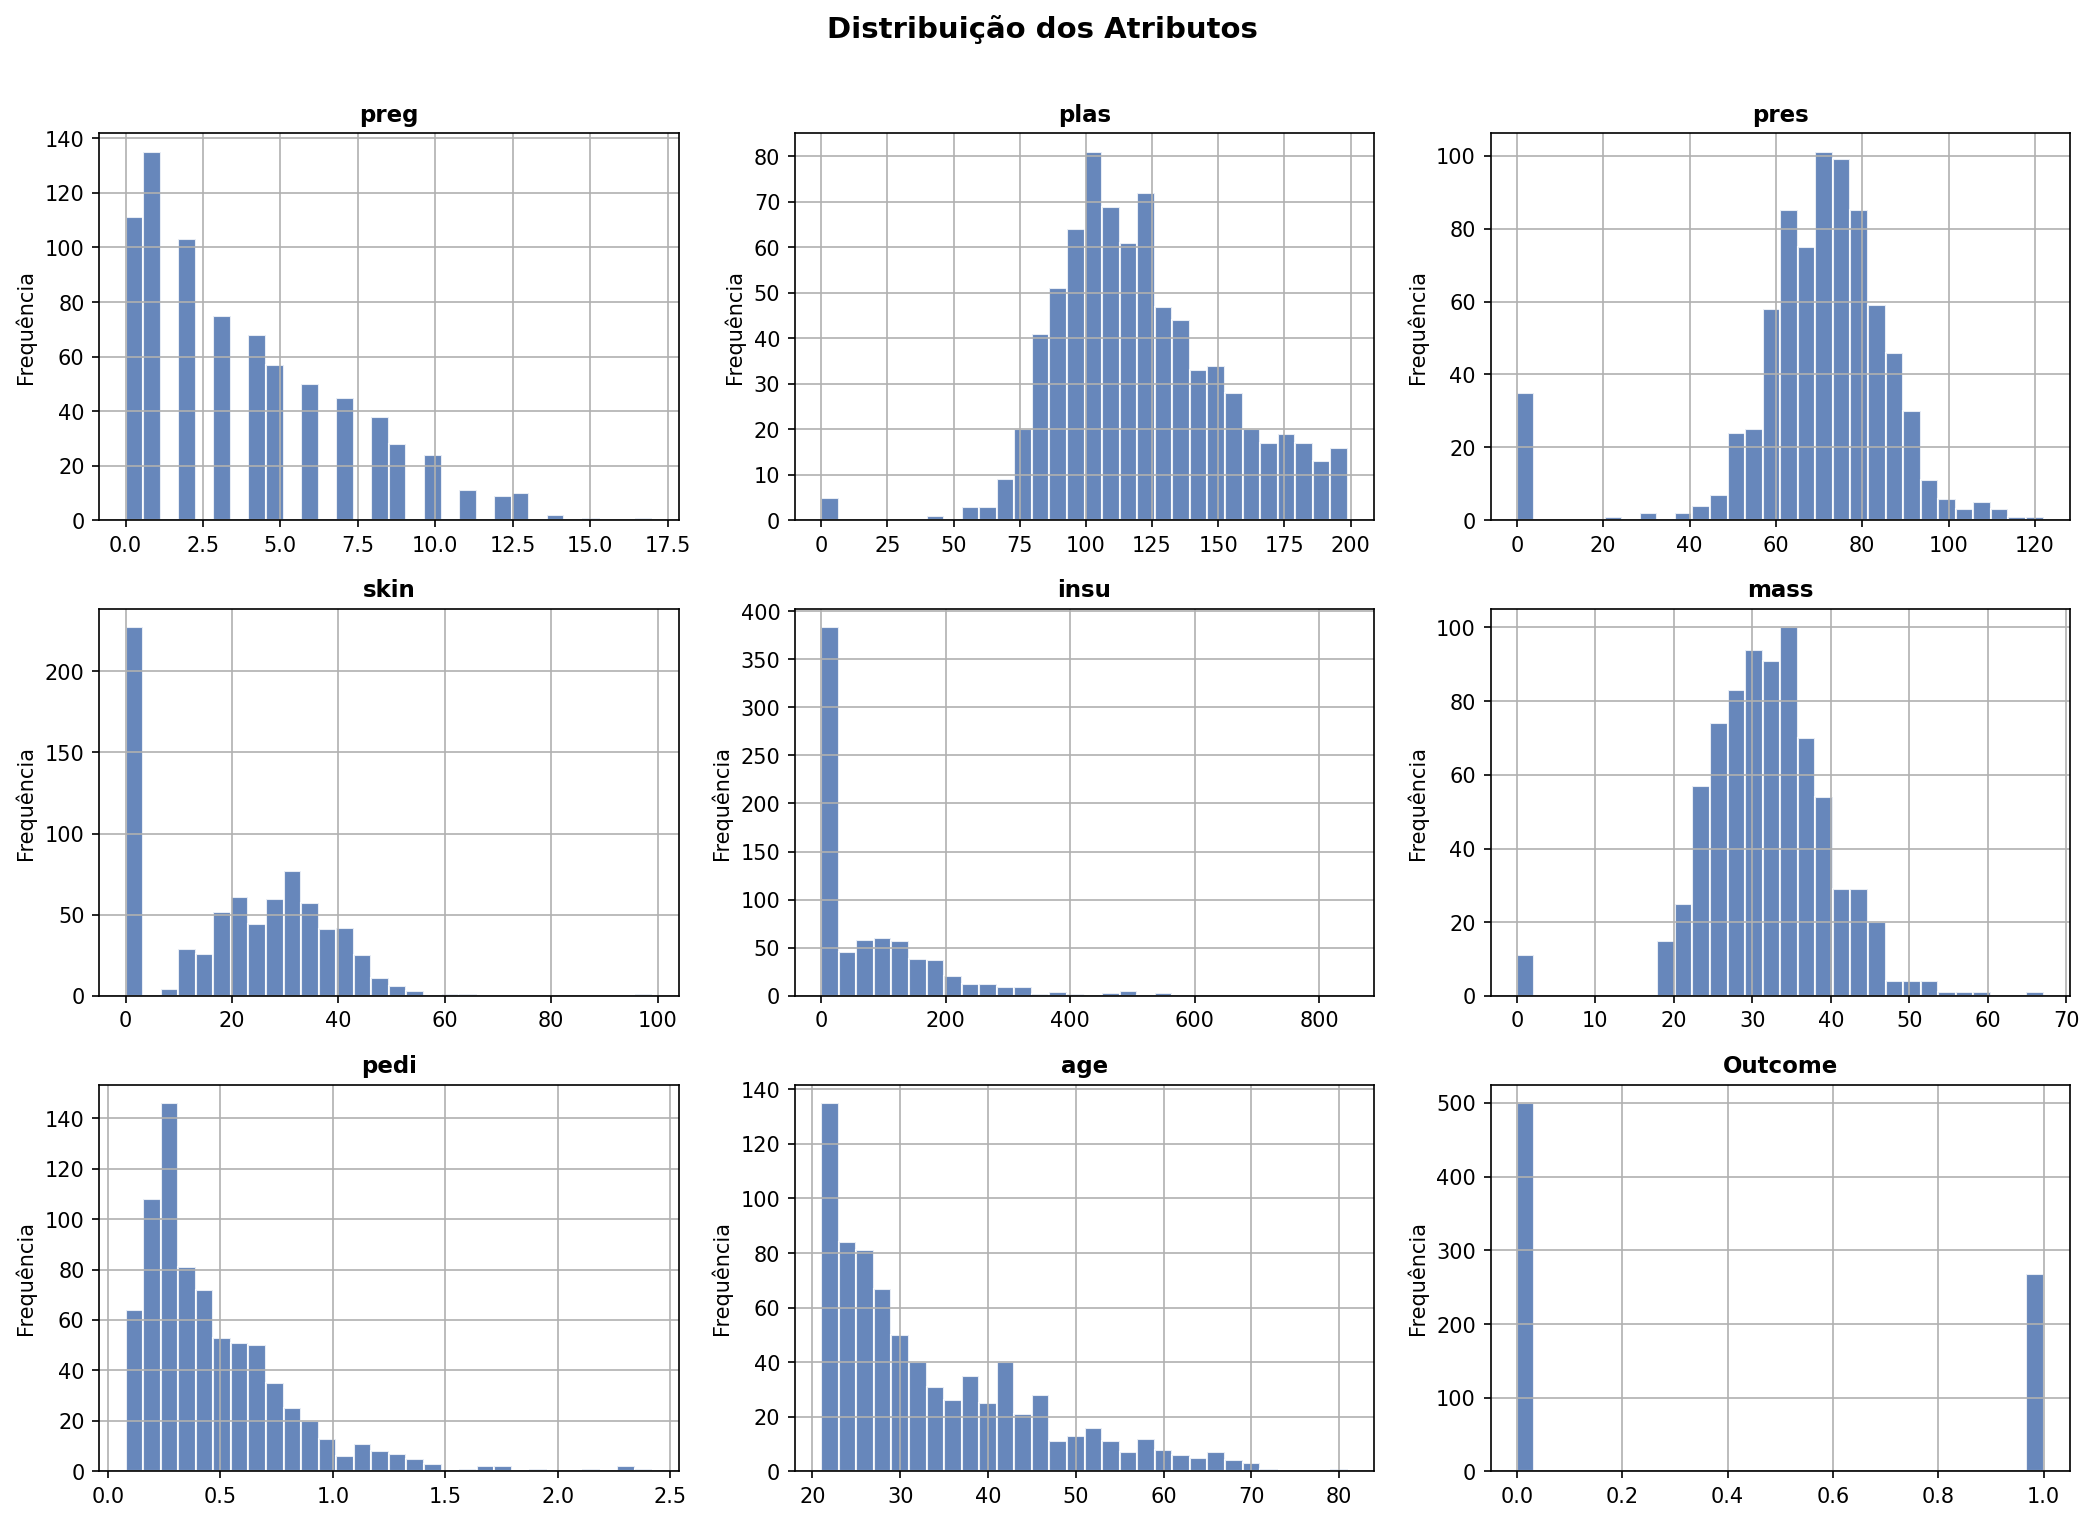
\includegraphics[width=\textwidth]{../output/01_distribuicoes.png}
\caption{Distribuição dos atributos do dataset.}
\end{figure}

A Figura 2 exibe os boxplots por classe (Outcome), evidenciando que variáveis como \texttt{plas}, \texttt{mass} e \texttt{age} apresentam distribuições visivelmente distintas entre as classes positiva e negativa, sugerindo poder discriminativo relevante.

\begin{figure}[ht]
\centering
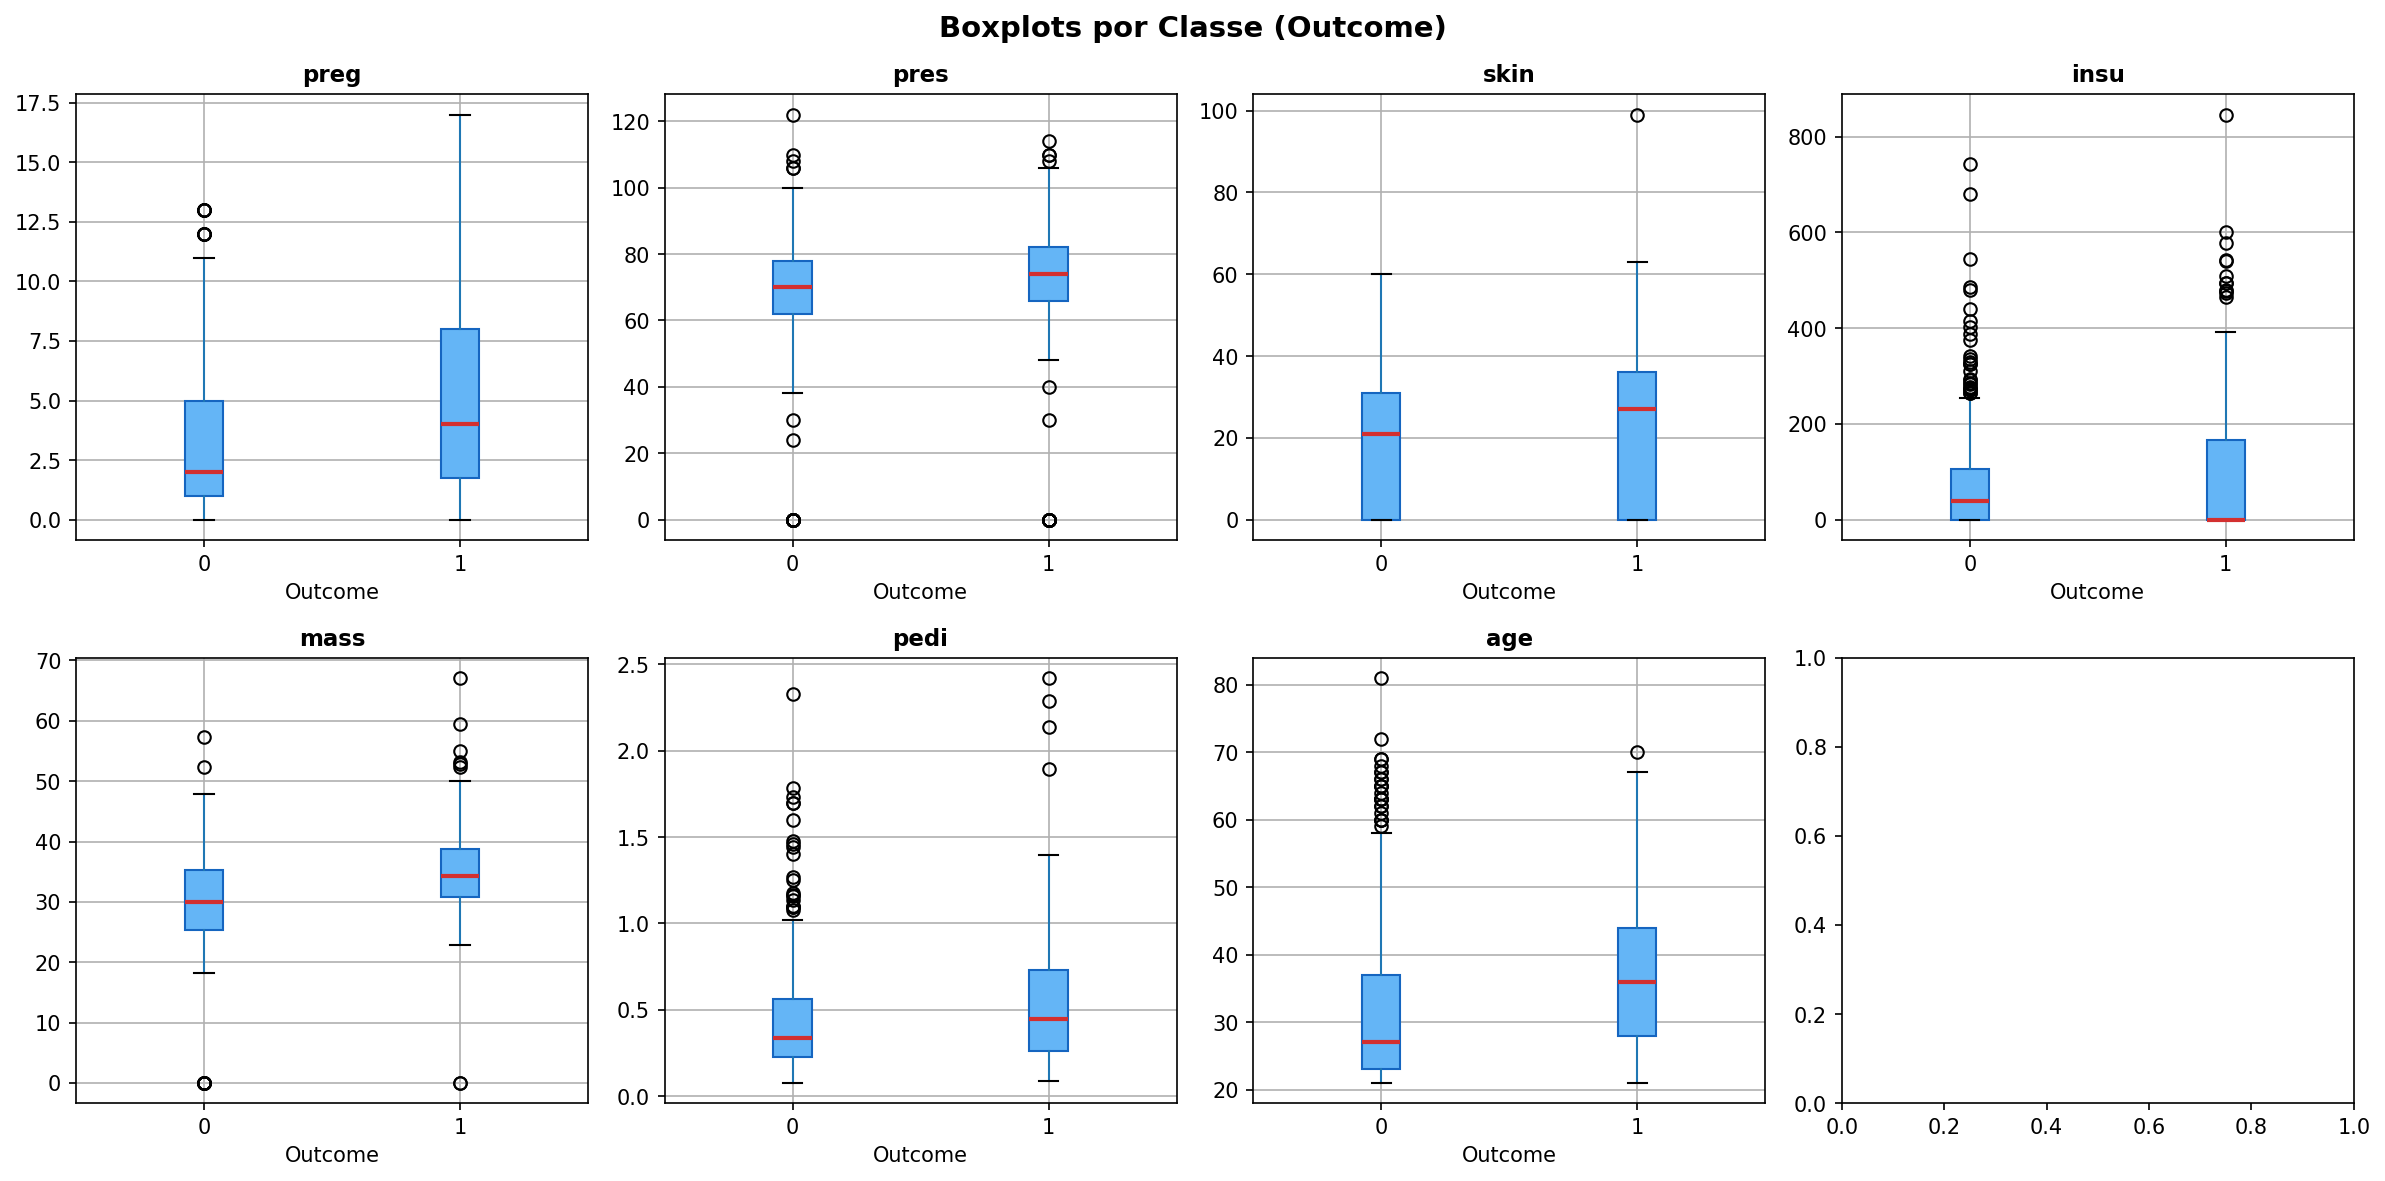
\includegraphics[width=\textwidth]{../output/02_boxplots_por_classe.png}
\caption{Boxplots dos atributos por classe (Outcome).}
\end{figure}

A Figura 3 apresenta a matriz de correlação de Pearson, na qual se observa a ausência de multicolinearidade severa (nenhum par com |r| $>$ 0,7). As correlações mais relevantes são entre \texttt{skin} e \texttt{insu} (r = 0,44) e entre \texttt{age} e \texttt{preg} (r = 0,54).

\begin{figure}[ht]
\centering
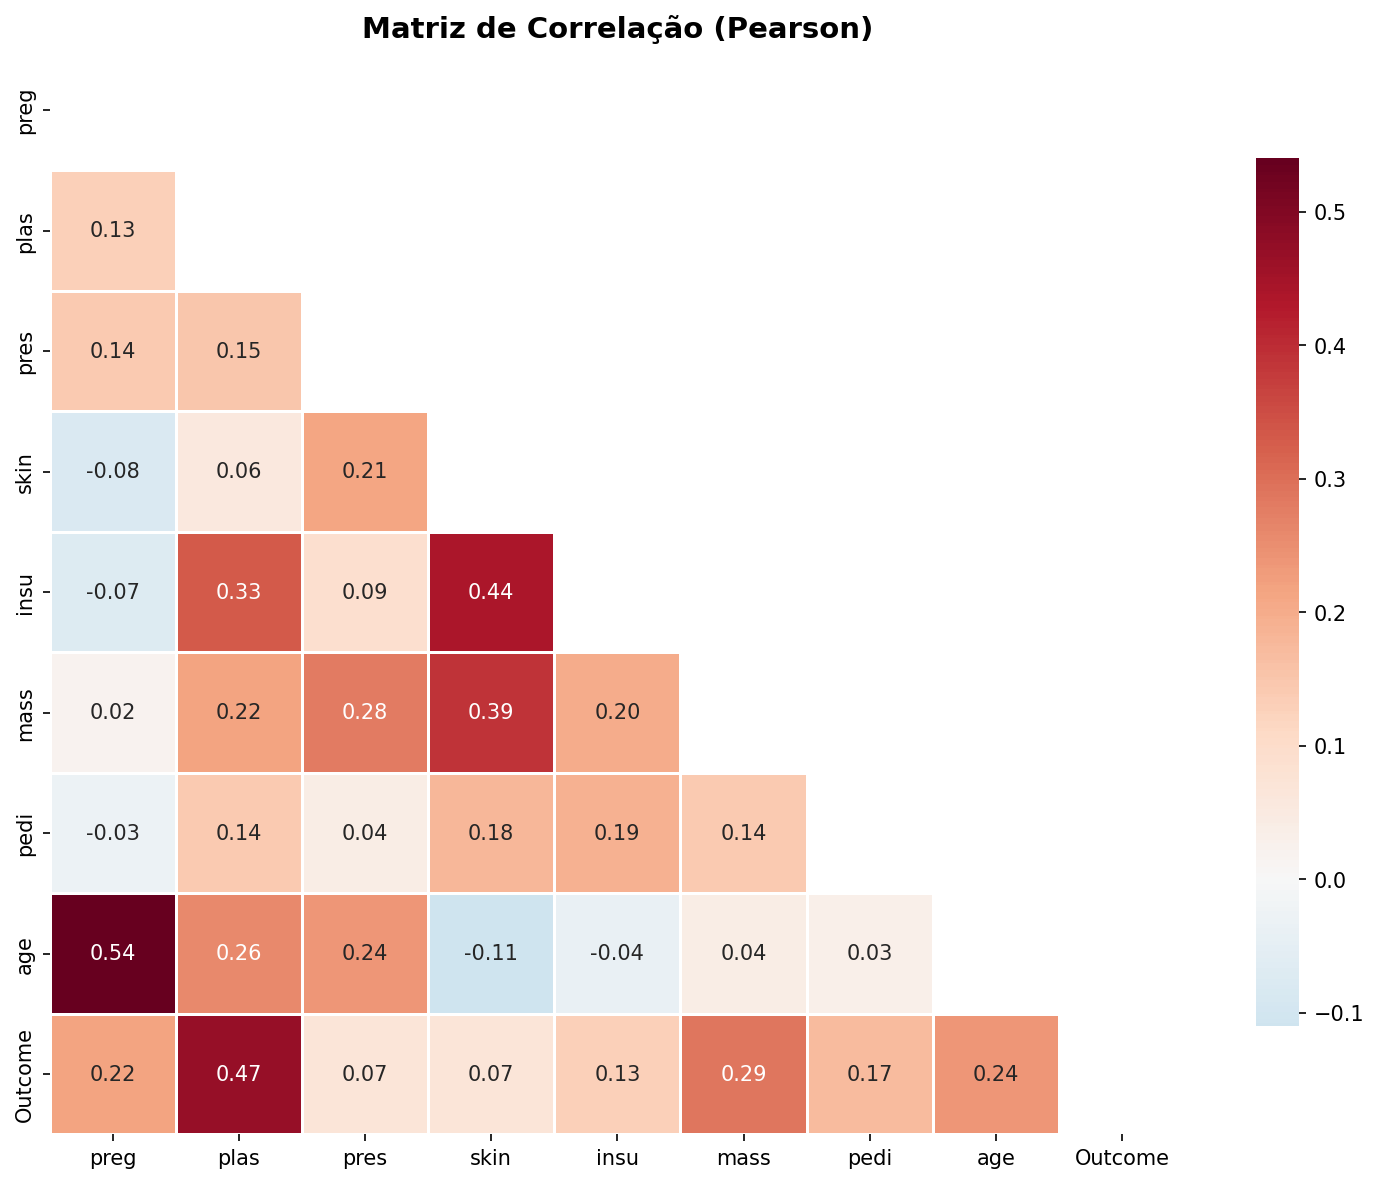
\includegraphics[width=\textwidth]{../output/03_correlacao.png}
\caption{Matriz de correlação de Pearson entre os atributos.}
\end{figure}

A variável de regressão (\texttt{plas}) apresenta distribuição com leve assimetria positiva, conforme ilustrado na Figura 4. O Q-Q Plot indica um desvio da normalidade nas caudas, especialmente na cauda superior.

\begin{figure}[ht]
\centering
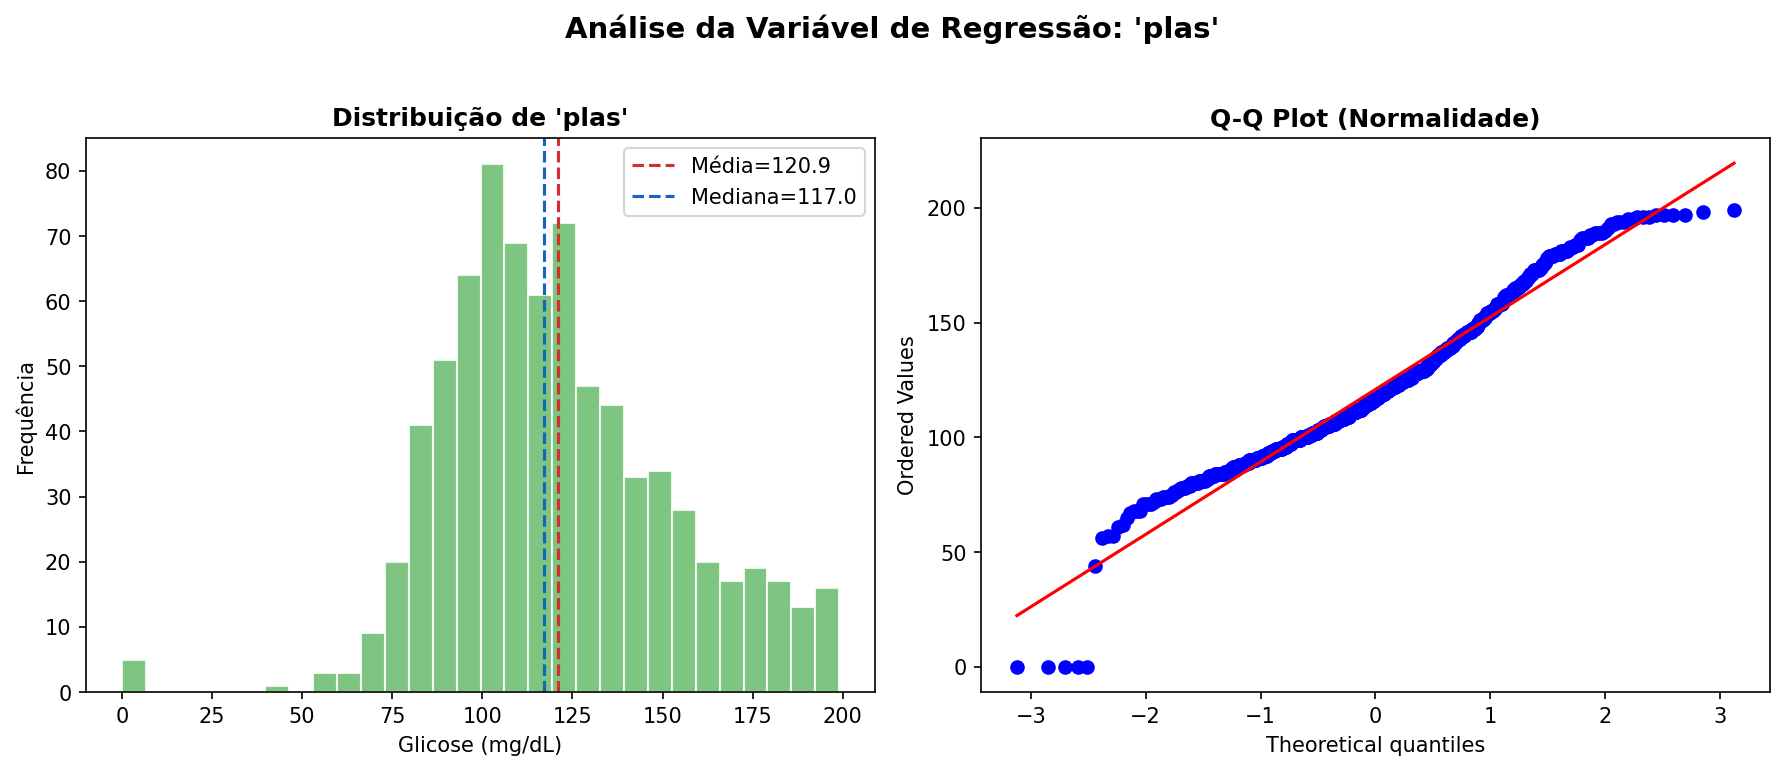
\includegraphics[width=\textwidth]{../output/04_regressao_target.png}
\caption{Análise da variável de regressão (glicose): distribuição e Q-Q Plot.}
\end{figure}

A distribuição da variável alvo de classificação binária é mostrada na Figura 5, com 500 amostras negativas e 268 positivas.

\begin{figure}[ht]
\centering
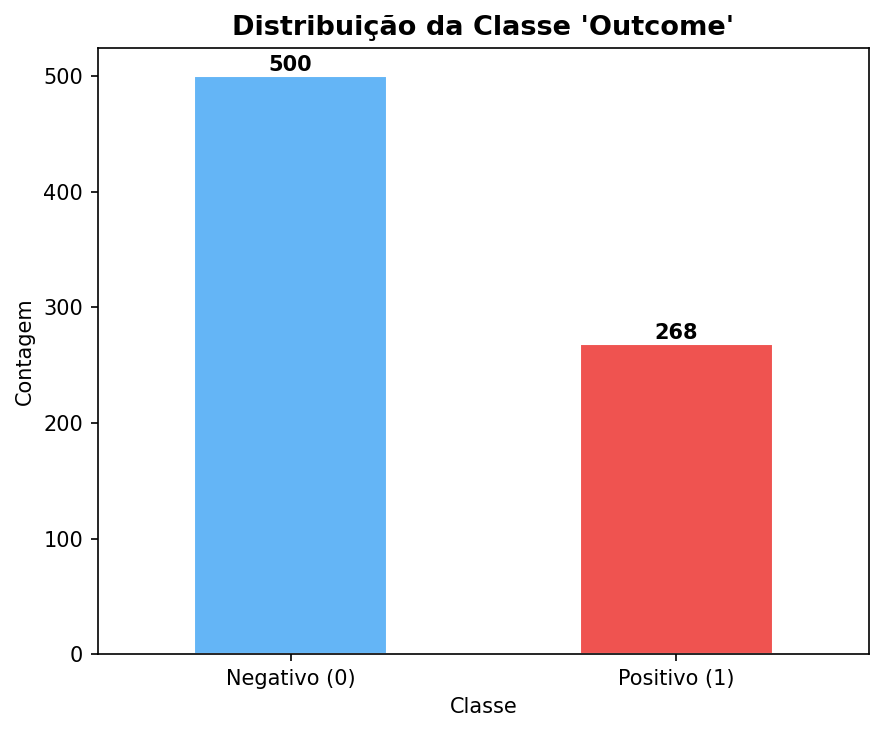
\includegraphics[width=\textwidth]{../output/05_distribuicao_classes.png}
\caption{Distribuição da classe alvo de classificação binária.}
\end{figure}

\subsection{Pré-processamento}

A Figura 6 compara as distribuições dos 5 atributos afetados antes (com zeros inválidos) e após a imputação por KNN. Observa-se que a imputação eliminou os picos artificiais em zero, especialmente visíveis em \texttt{insu} e \texttt{skin}, preservando a forma geral das distribuições.

\begin{figure}[ht]
\centering
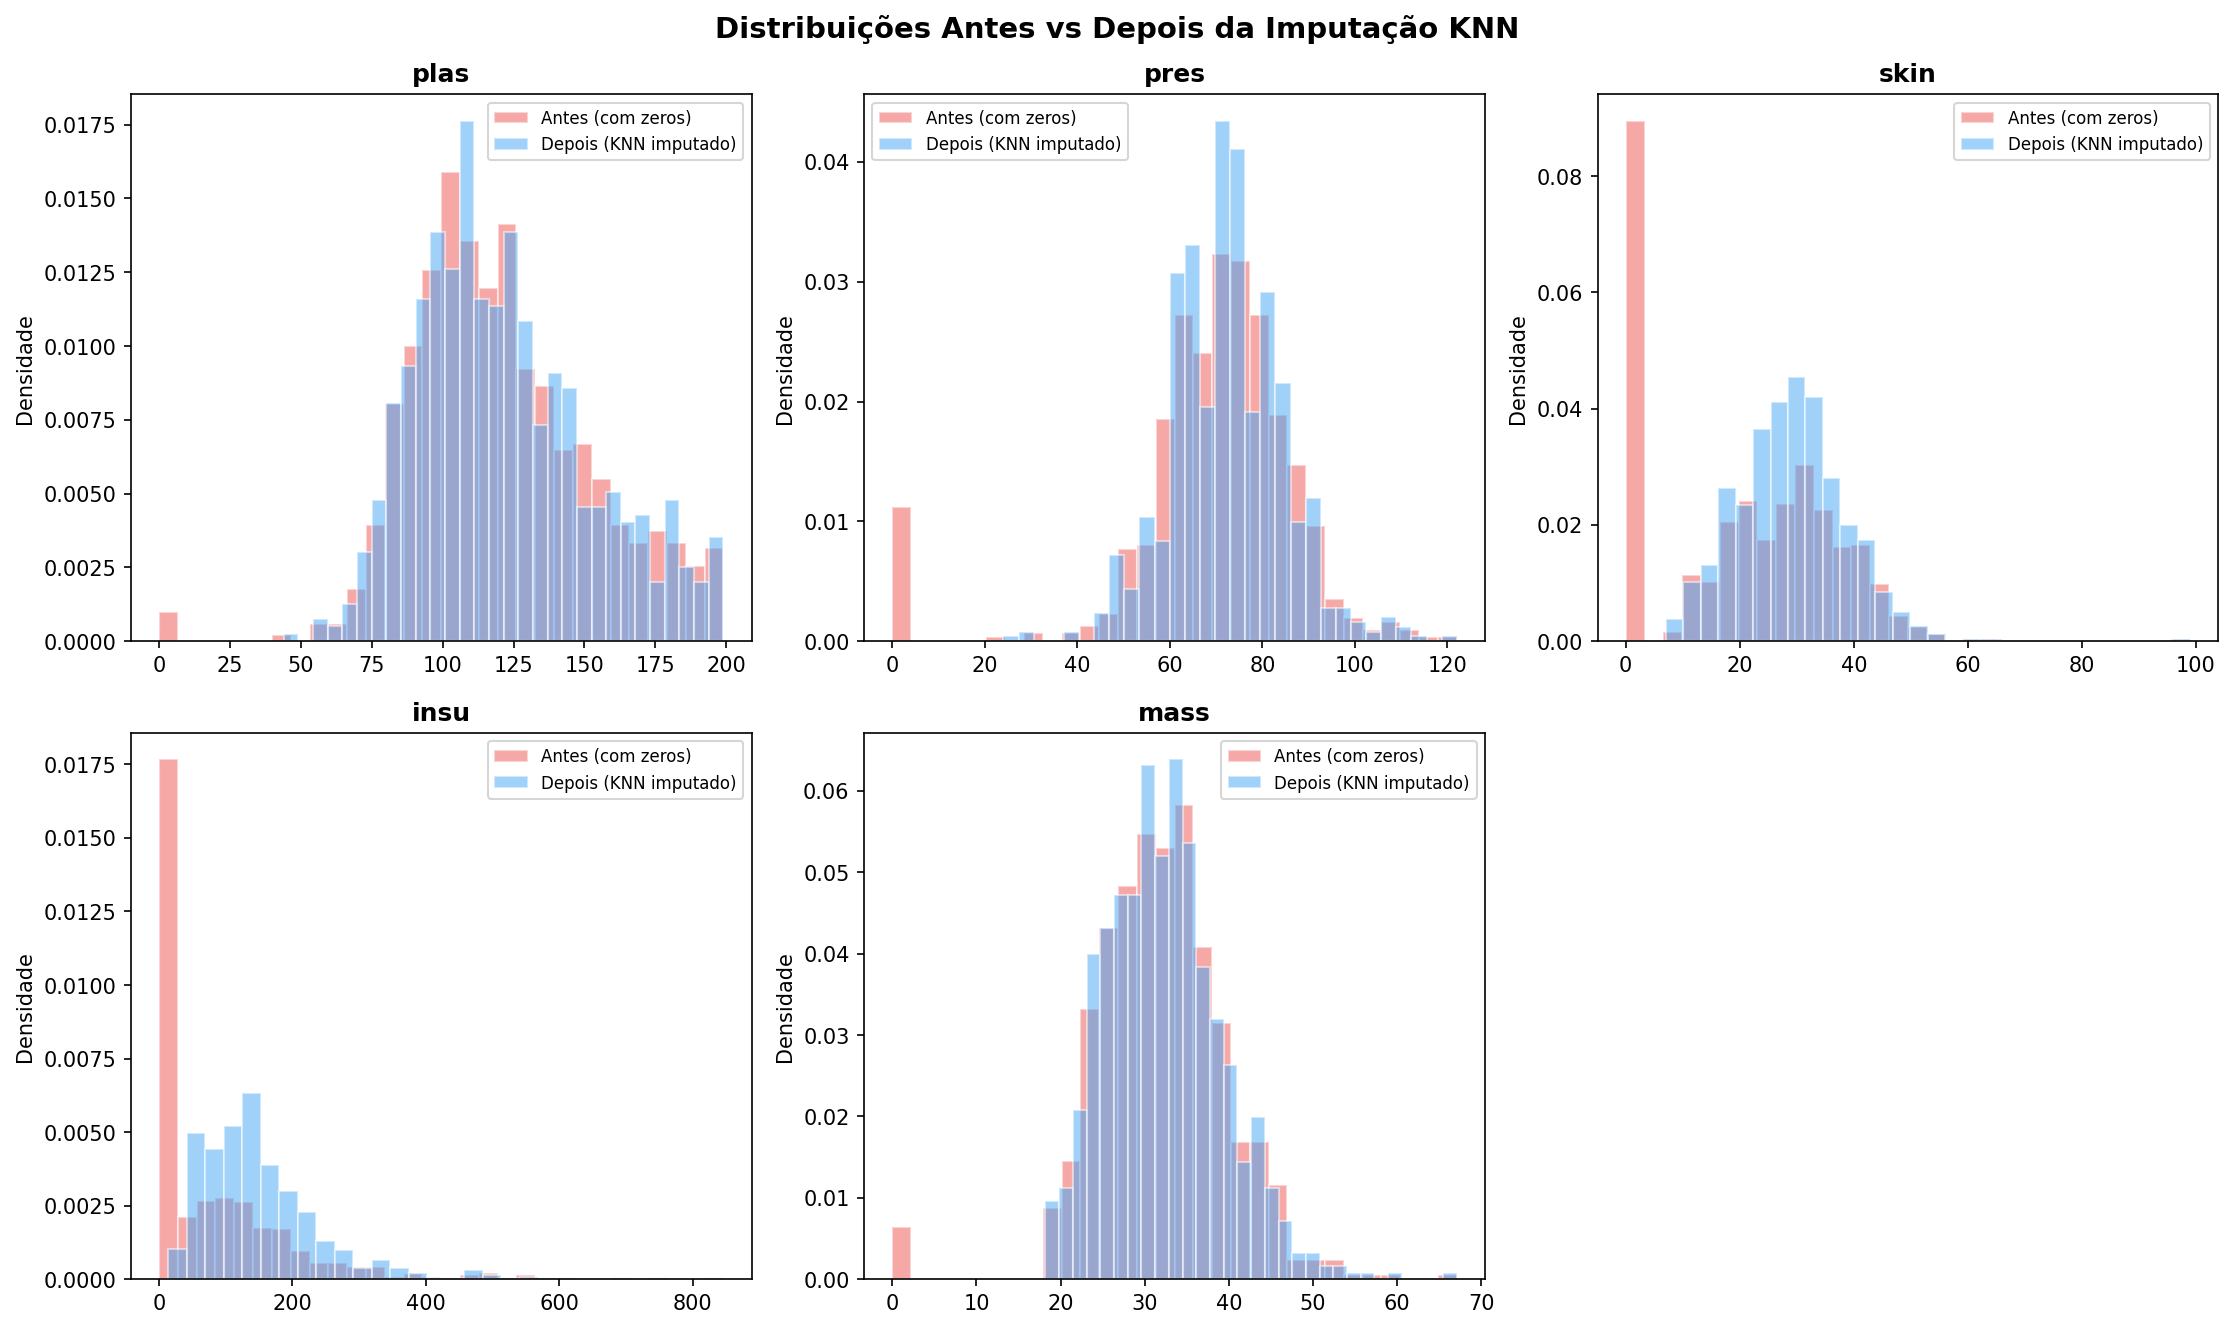
\includegraphics[width=\textwidth]{../output/06_imputacao_antes_depois.png}
\caption{Distribuições antes e depois da imputação KNN.}
\end{figure}

A Figura 7 apresenta os boxplots antes e após o escalonamento com RobustScaler. Após o escalonamento, todas as features estão centradas na mediana (valor 0) com dispersão proporcional ao IQR, permitindo que algoritmos sensíveis à escala (como MLPs e SVMs) operem de forma adequada.

\begin{figure}[ht]
\centering
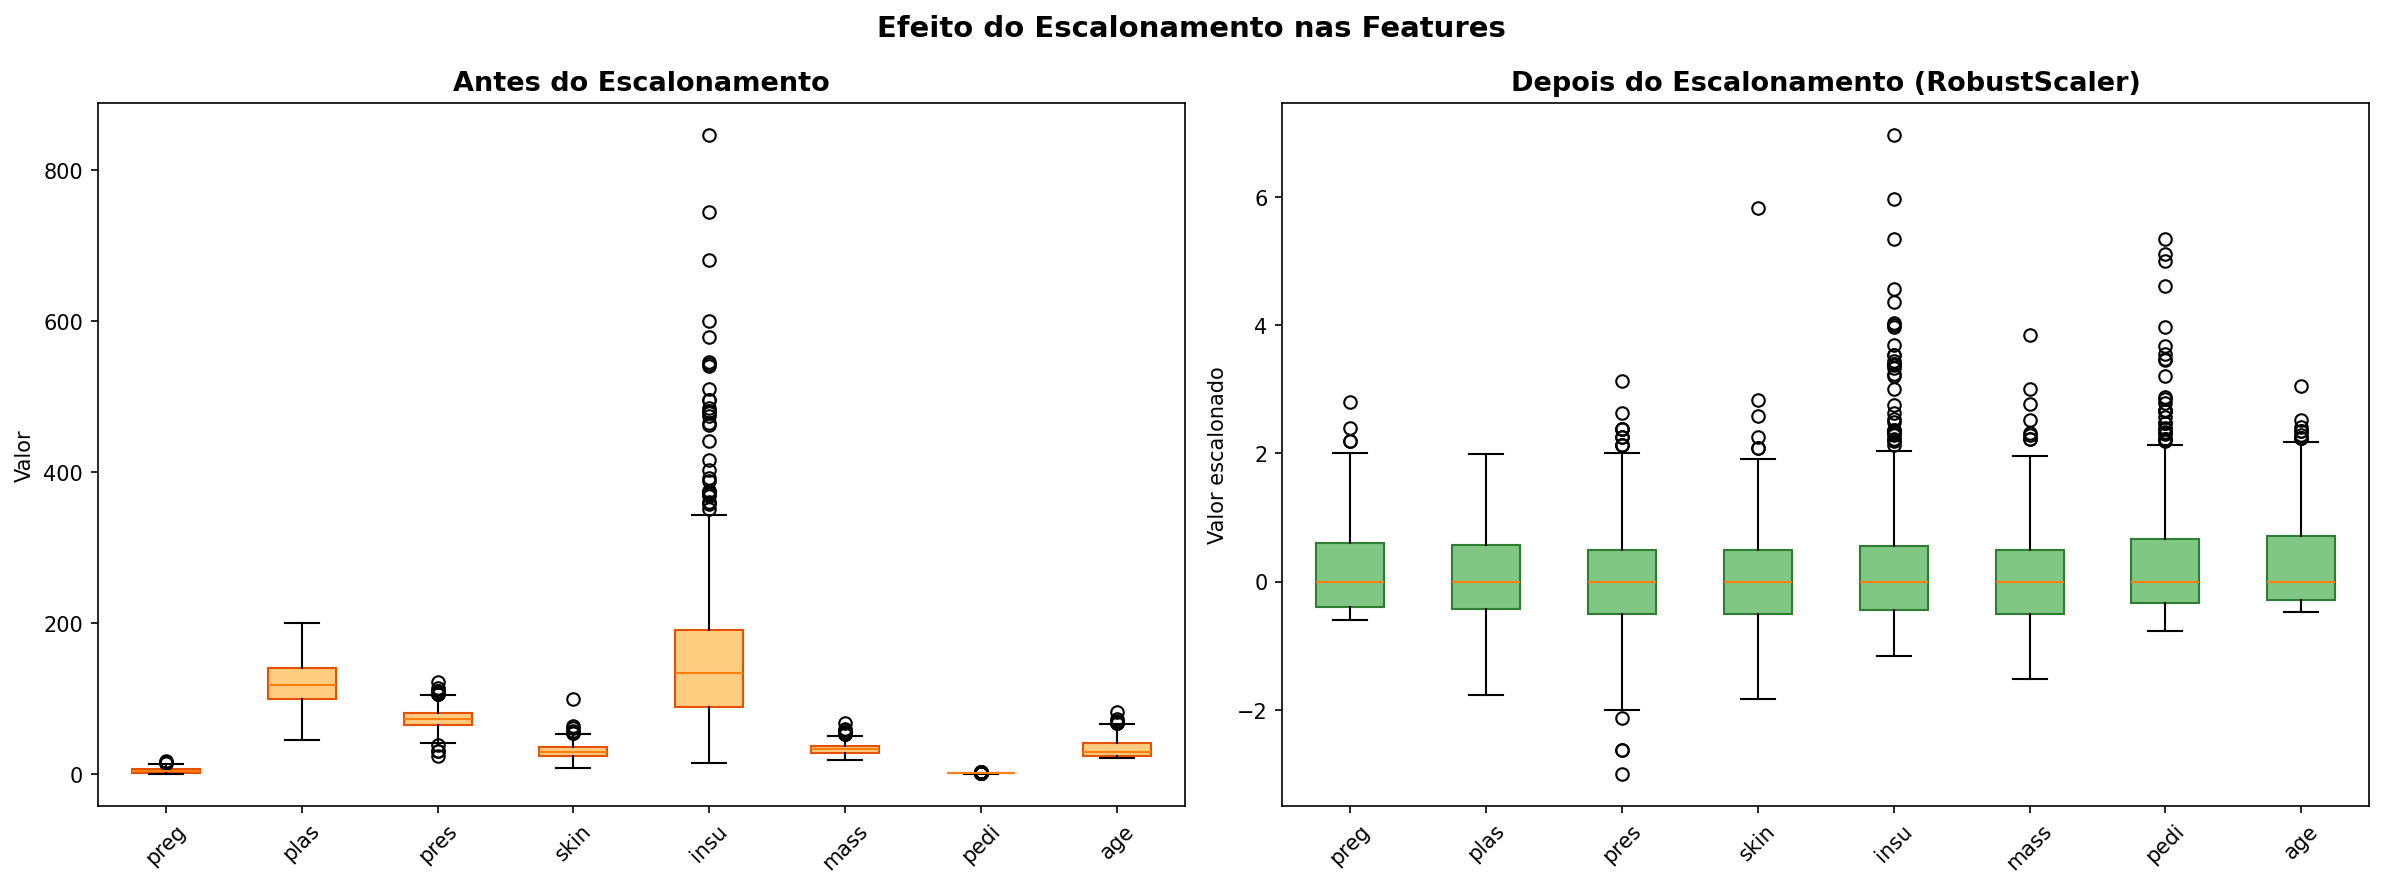
\includegraphics[width=\textwidth]{../output/07_escalonamento_antes_depois.png}
\caption{Boxplots antes e após o escalonamento com RobustScaler.}
\end{figure}

A Figura 8 exibe a matriz de correlação pós-processamento, confirmando que as relações estruturais entre os atributos foram preservadas pelo pipeline de pré-processamento.

\begin{figure}[ht]
\centering
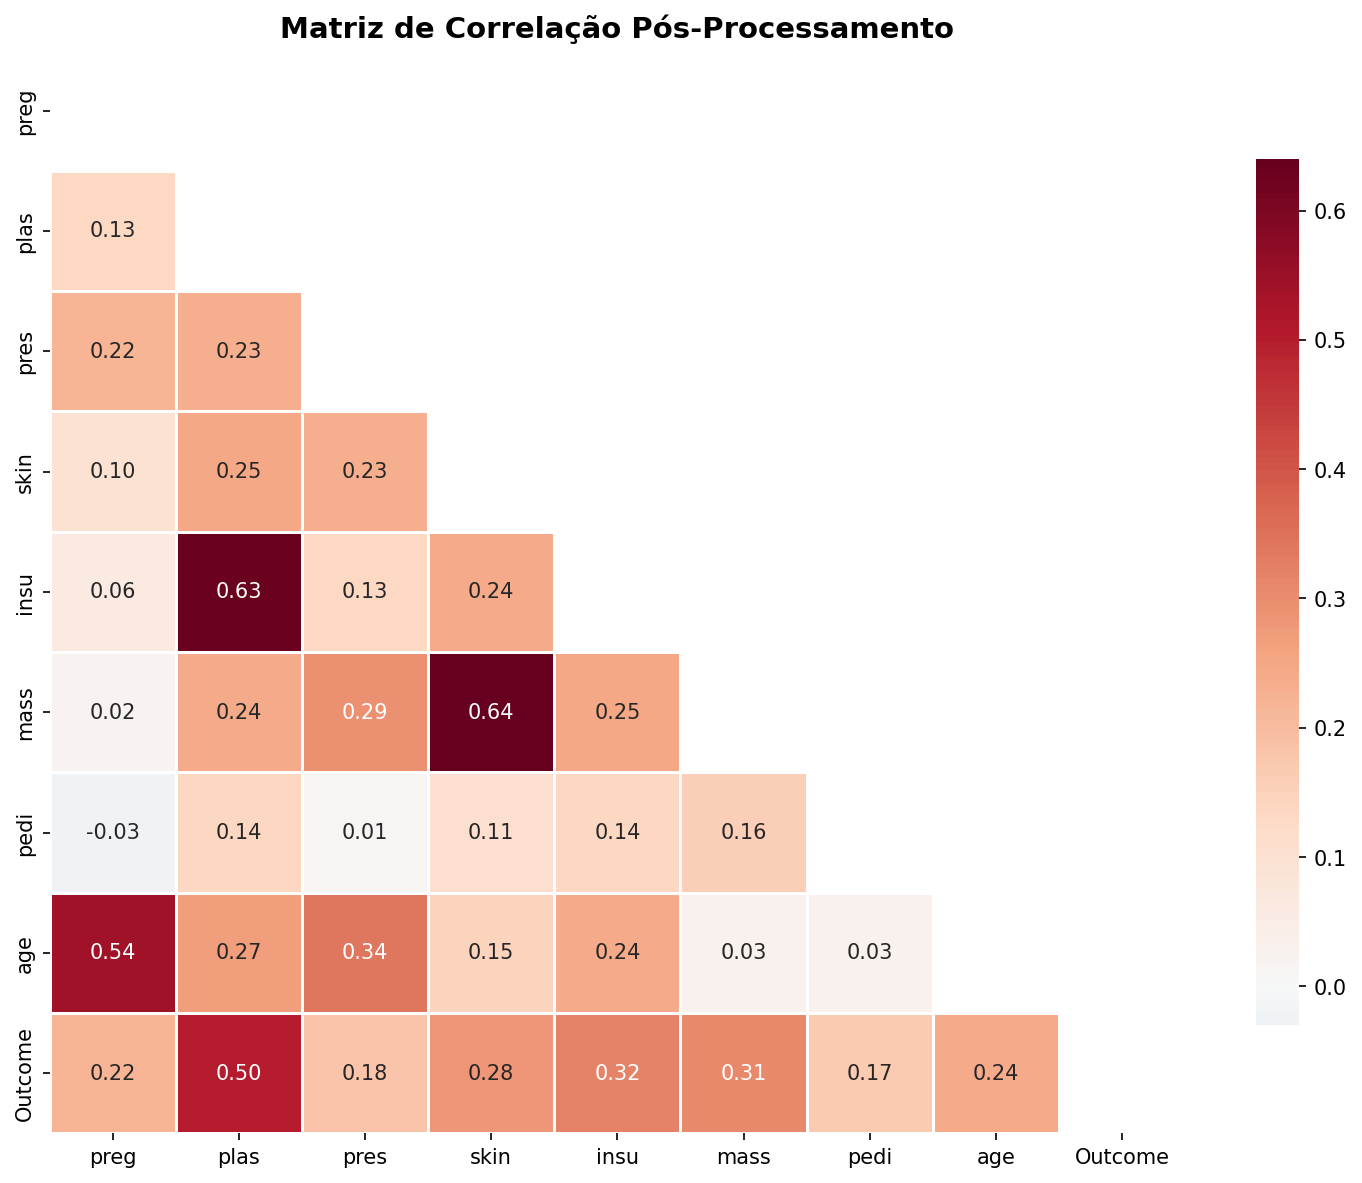
\includegraphics[width=\textwidth]{../output/08_correlacao_pos_processamento.png}
\caption{Matriz de correlação de Pearson pós-processamento.}
\end{figure}

\subsection{Seleção de Features e Interpretabilidade}

\subsubsection{Análise SHAP --- Importância Global}

A Figura 9 apresenta o SHAP Summary Plot (beeswarm), que exibe a distribuição dos valores SHAP para cada feature ao longo de todas as amostras. Valores SHAP positivos empurram a predição em direção à classe positiva (diabética), enquanto valores negativos empurram em direção à classe negativa.

\begin{figure}[ht]
\centering
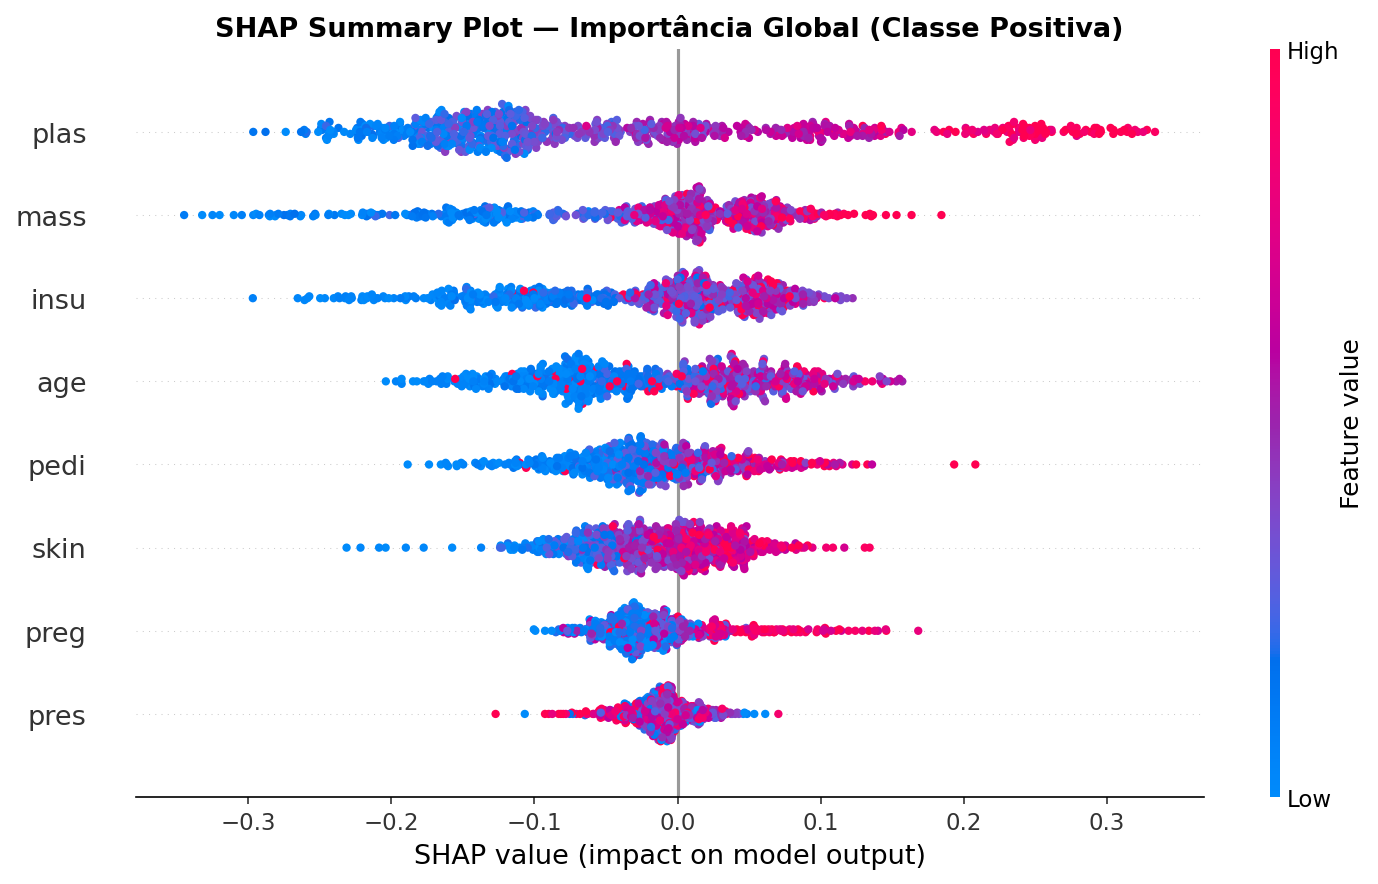
\includegraphics[width=\textwidth]{../output/09_shap_summary_beeswarm.png}
\caption{SHAP Summary Plot: importância global das features para a classe positiva.}
\end{figure}

A Figura 10 complementa a análise com o SHAP Bar Plot, que mostra a importância média absoluta de cada atributo.

\begin{figure}[ht]
\centering
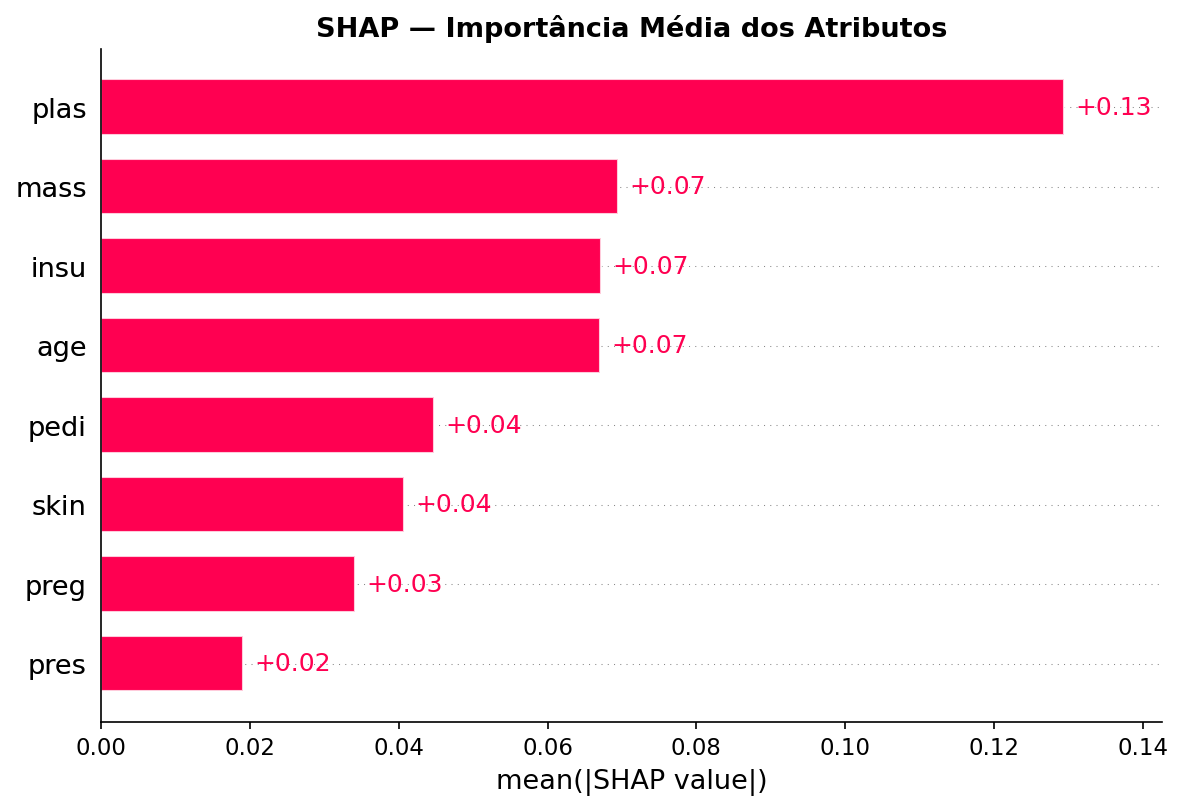
\includegraphics[width=\textwidth]{../output/10_shap_bar_importance.png}
\caption{SHAP Bar Plot: importância média dos atributos.}
\end{figure}

\subsubsection{Explicação Local --- Predições Individuais}

As Figuras 11 e 12 apresentam os waterfall plots do SHAP para uma amostra da classe positiva e uma da classe negativa, respectivamente. Esses gráficos decompõem a predição individual em contribuições aditivas de cada feature, partindo do valor base (predição média do modelo) até a predição final.

\begin{figure}[ht]
\centering
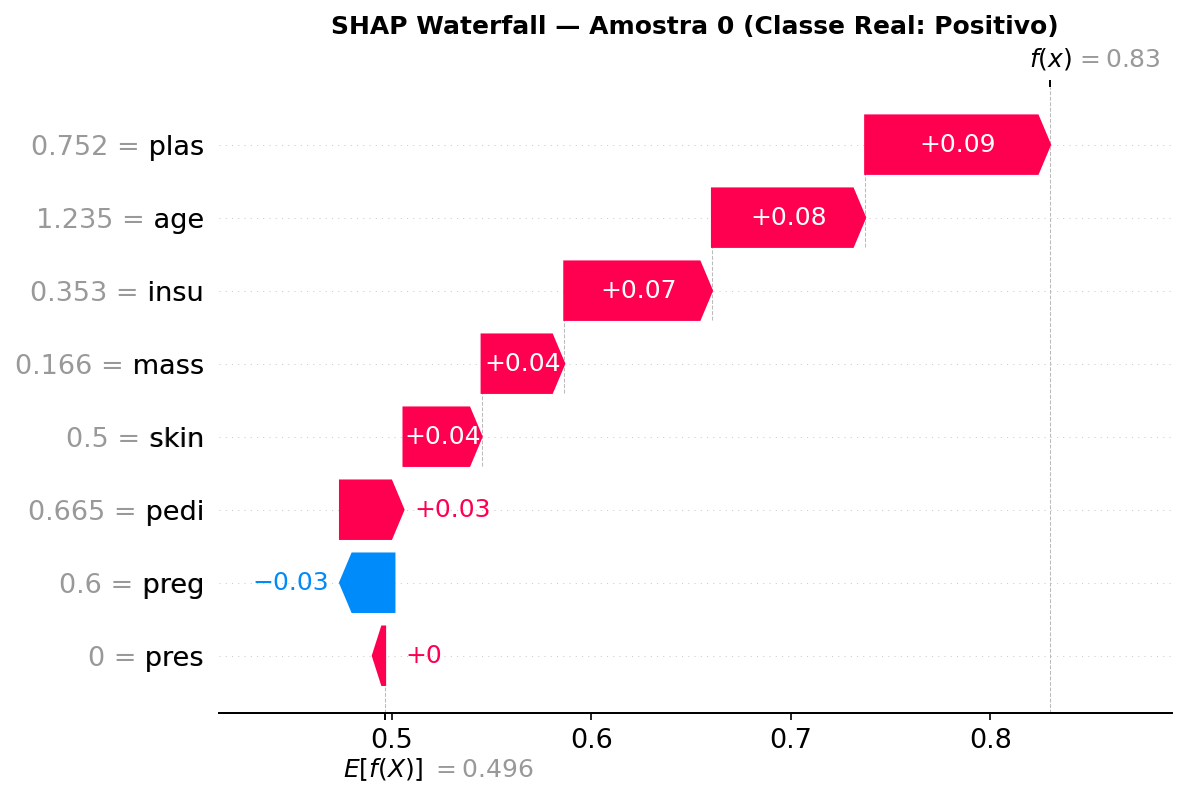
\includegraphics[width=\textwidth]{../output/11_shap_waterfall_positivo.png}
\caption{SHAP Waterfall: explicação local de uma amostra positiva (diabética).}
\end{figure}

\begin{figure}[ht]
\centering
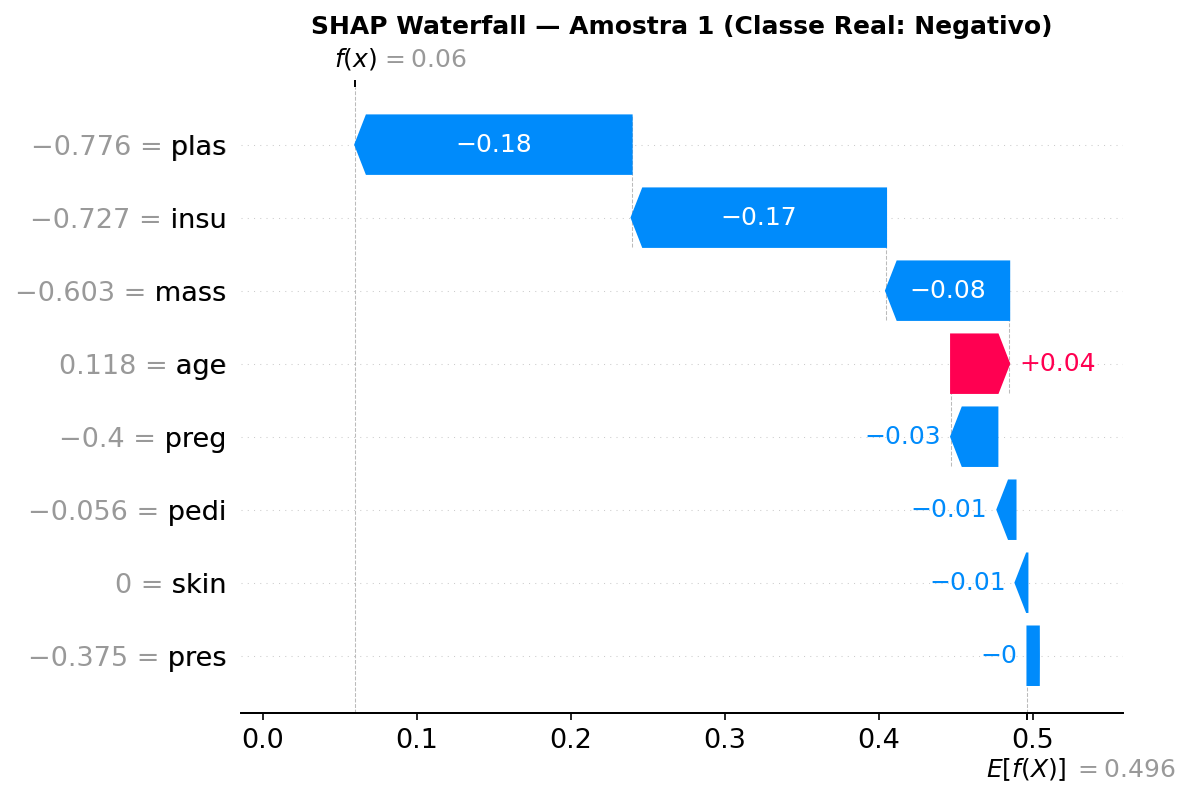
\includegraphics[width=\textwidth]{../output/12_shap_waterfall_negativo.png}
\caption{SHAP Waterfall: explicação local de uma amostra negativa (não diabética).}
\end{figure}

\subsubsection{Comparação MI vs. SHAP}

A Figura 13 exibe lado a lado os rankings de importância gerados pela Informação Mútua e pelo SHAP. As barras coloridas representam as features selecionadas pela MI (acima do limiar), enquanto as barras cinzas representam as features descartadas.

\begin{figure}[ht]
\centering
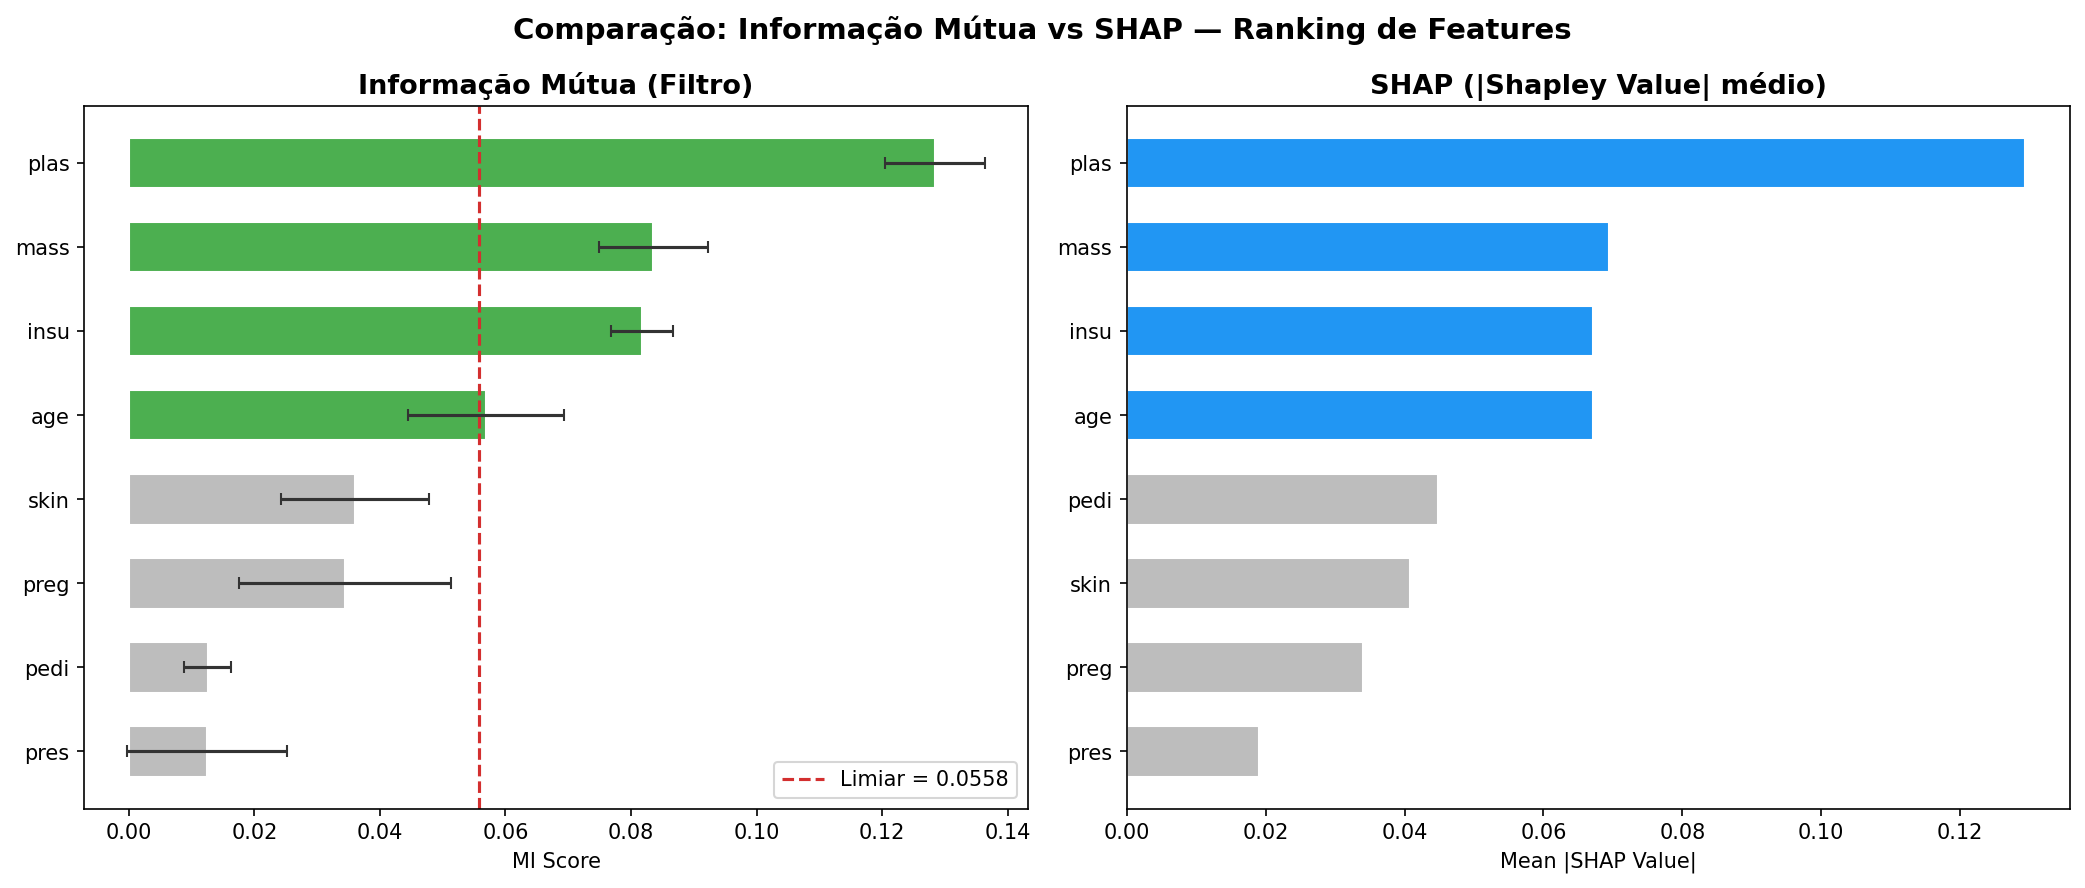
\includegraphics[width=\textwidth]{../output/13_mi_vs_shap_ranking.png}
\caption{Comparação dos rankings de importância: Informação Mútua vs. SHAP.}
\end{figure}

A concordância entre os dois métodos foi avaliada por meio da correlação de Spearman entre os rankings. O coeficiente obtido foi \textbf{$\rho$ = 0,9286 (p = 0,0009)}, indicando concordância muito alta e estatisticamente significativa entre os dois métodos. As três features globalmente selecionadas pela MI (\texttt{plas}, \texttt{insu}, \texttt{mass}) pertencem simultaneamente ao topo do ranking SHAP, corroborando a validade da seleção.

\subsubsection{Impacto da Seleção de Features (MI dentro da CV)}

A Figura 14 apresenta a comparação de desempenho entre os dois cenários, com a seleção MI realizada \textbf{dentro de cada fold} para garantir ausência de data leakage.

\begin{figure}[ht]
\centering
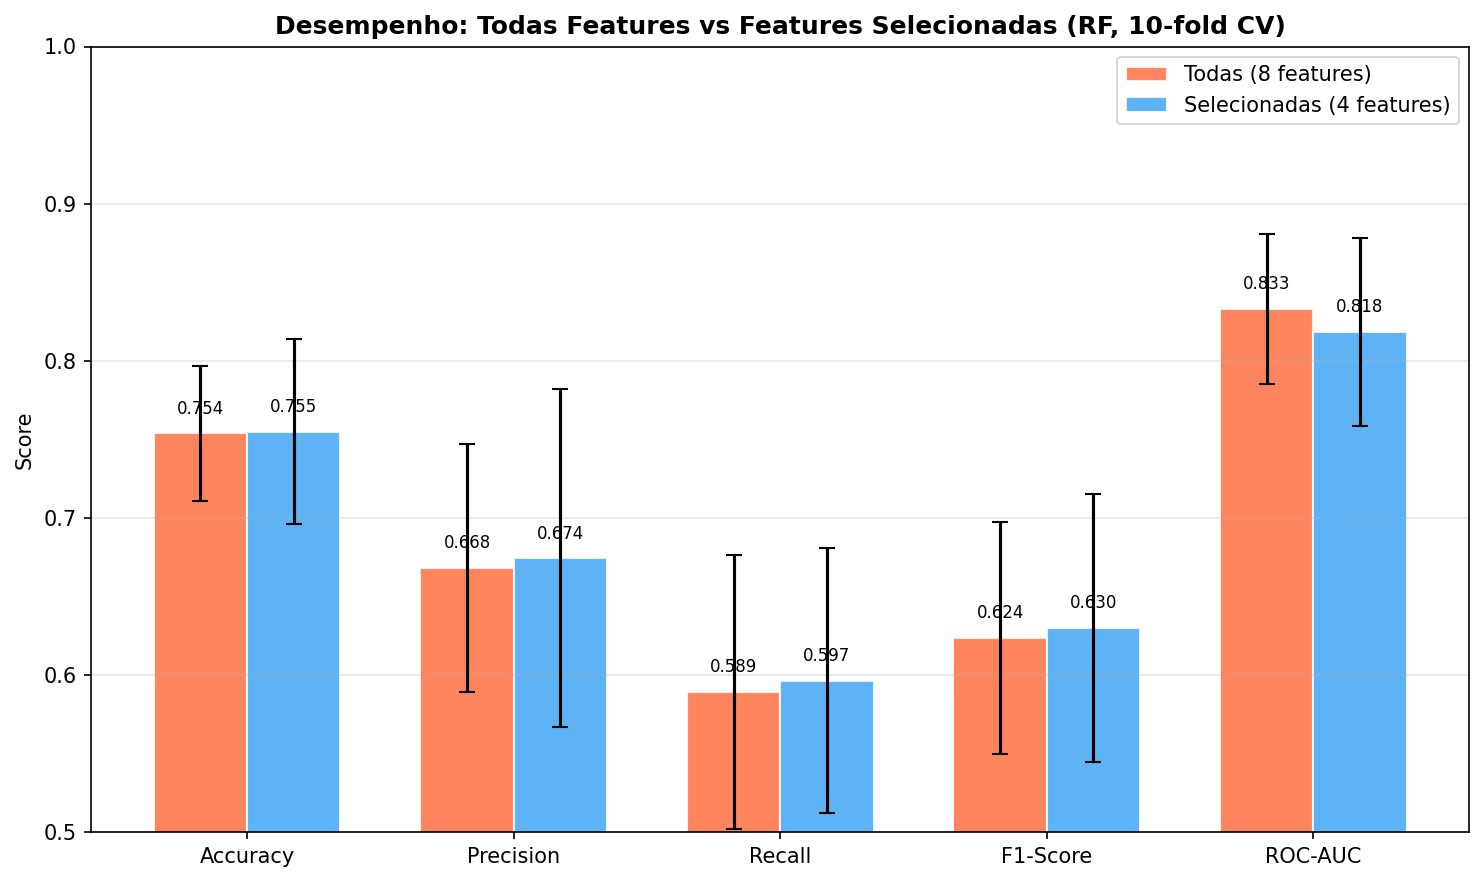
\includegraphics[width=\textwidth]{../output/14_desempenho_comparativo.png}
\caption{Desempenho comparativo: todas as features vs. features selecionadas (RF, 10-fold CV).}
\end{figure}

\textbf{Consistência da seleção por fold:} As features \texttt{plas}, \texttt{insu} e \texttt{mass} foram selecionadas em todos os 10 folds (10/10), confirmando que são atributos robustamente relevantes independentemente da partição dos dados. A feature \texttt{age} foi selecionada em apenas 2/10 folds, evidenciando que sua relevância é limítrofe e sensível à composição dos dados de treino.

\textbf{Métricas comparativas (10-fold CV estratificada):}

\begin{table}[ht]
\centering
\begin{tabularx}{\textwidth}{|l|X|X|X|}
\hline
Métrica & Todas (8 feat.) & Selecionadas (3 feat.) & $\Delta$ \\
\hline
Accuracy & 0,7476 $\pm$ 0,0478 & 0,7297 $\pm$ 0,0430 & $-$0,0179 \\
\hline
Precision & 0,6338 $\pm$ 0,0729 & 0,6080 $\pm$ 0,0634 & $-$0,0258 \\
\hline
Recall & 0,6636 $\pm$ 0,0710 & 0,6500 $\pm$ 0,0676 & $-$0,0136 \\
\hline
F1-Score & 0,6471 $\pm$ 0,0658 & 0,6264 $\pm$ 0,0539 & $-$0,0207 \\
\hline
ROC-AUC & 0,8259 $\pm$ 0,0488 & 0,7957 $\pm$ 0,0380 & $-$0,0302 \\
\hline
\end{tabularx}
\end{table}


\textbf{Gap de overfitting (acurácia treino $-$ teste):}
\begin{itemize}
\item Todas as features: \textbf{0,2521}
\item Features selecionadas: \textbf{0,2694}

\end{itemize}
Os resultados, agora avaliados sem data leakage, revelam um quadro mais realista: o modelo com 3 features selecionadas apresenta desempenho ligeiramente inferior ao modelo com todas as 8 features em todas as métricas. Isso é esperado --- a avaliação anterior (com MI calculada fora da CV) inflava artificialmente as métricas do cenário selecionado ao permitir que a escolha das features considerasse os dados de validação. Com a seleção dentro da CV, o resultado é metodologicamente correto.

A diferença de ROC-AUC ($-$0,0302) e de Accuracy ($-$0,0179) é pequena em termos absolutos, e o desvio padrão reduzido no cenário selecionado indica maior estabilidade entre os folds. O gap de overfitting ligeiramente maior no cenário selecionado (0,2694 vs 0,2521) sugere que as 3 features, por serem mais informativas, permitem que o Random Forest ajuste-se mais agressivamente ao treino. Ainda assim, a redução de 62,5\% no número de atributos (de 8 para 3) com perda de desempenho inferior a 4\% em todas as métricas justifica a seleção sob a perspectiva de \textbf{interpretabilidade e eficiência computacional}.

\subsection{Classificação Binária com MLP}

\subsubsection{Curvas de Aprendizado}

A Figura 15 apresenta as curvas de aprendizado da MLP de classificação binária. O painel esquerdo mostra a evolução da perda (loss) por época no conjunto de treino e a métrica complementar no conjunto de validação. O painel direito exibe a evolução da acurácia de validação, com a linha pontilhada indicando o melhor valor obtido.

\begin{figure}[ht]
\centering
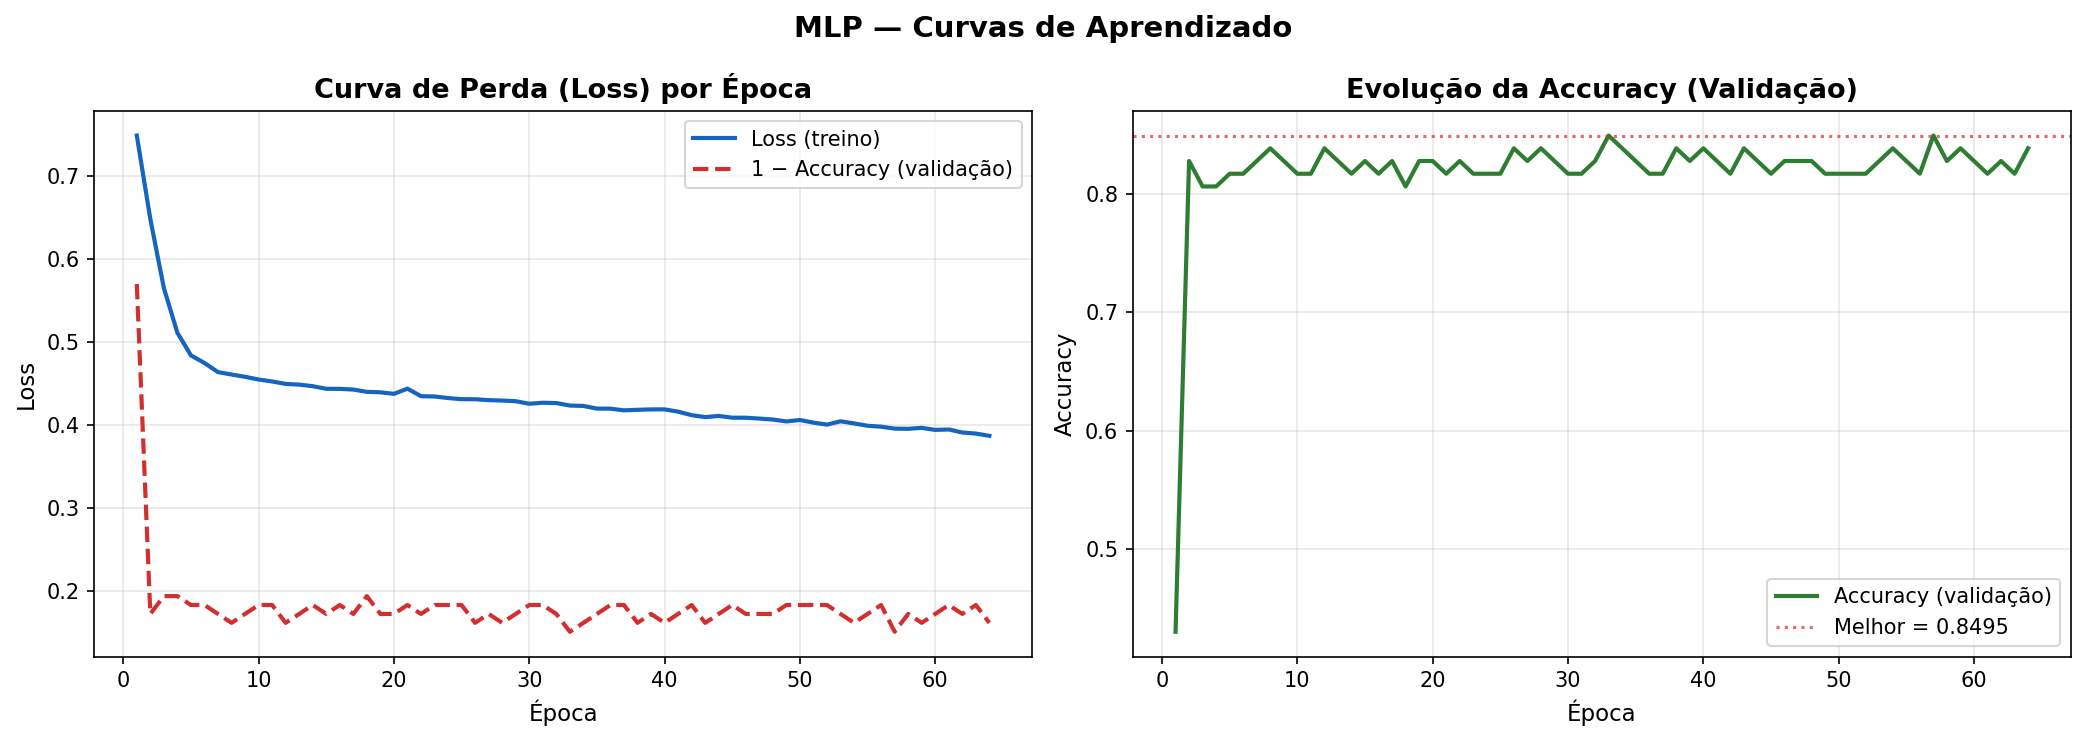
\includegraphics[width=\textwidth]{../output/15_mlp_curvas_aprendizado.png}
\caption{MLP de classificação binária: curvas de aprendizado (loss e accuracy por época).}
\end{figure}

As curvas indicam convergência estável, com a perda de treino decrescendo de forma monotônica e a acurácia de validação estabilizando após um número moderado de épocas. O early stopping interrompeu o treinamento no ponto adequado, evitando a degradação do desempenho de validação.

\subsubsection{Matrizes de Confusão}

A Figura 16 apresenta as matrizes de confusão dos três modelos avaliados (MLP, XGBoost e SVM), permitindo a comparação visual do número de verdadeiros positivos, verdadeiros negativos, falsos positivos e falsos negativos.

\begin{figure}[ht]
\centering
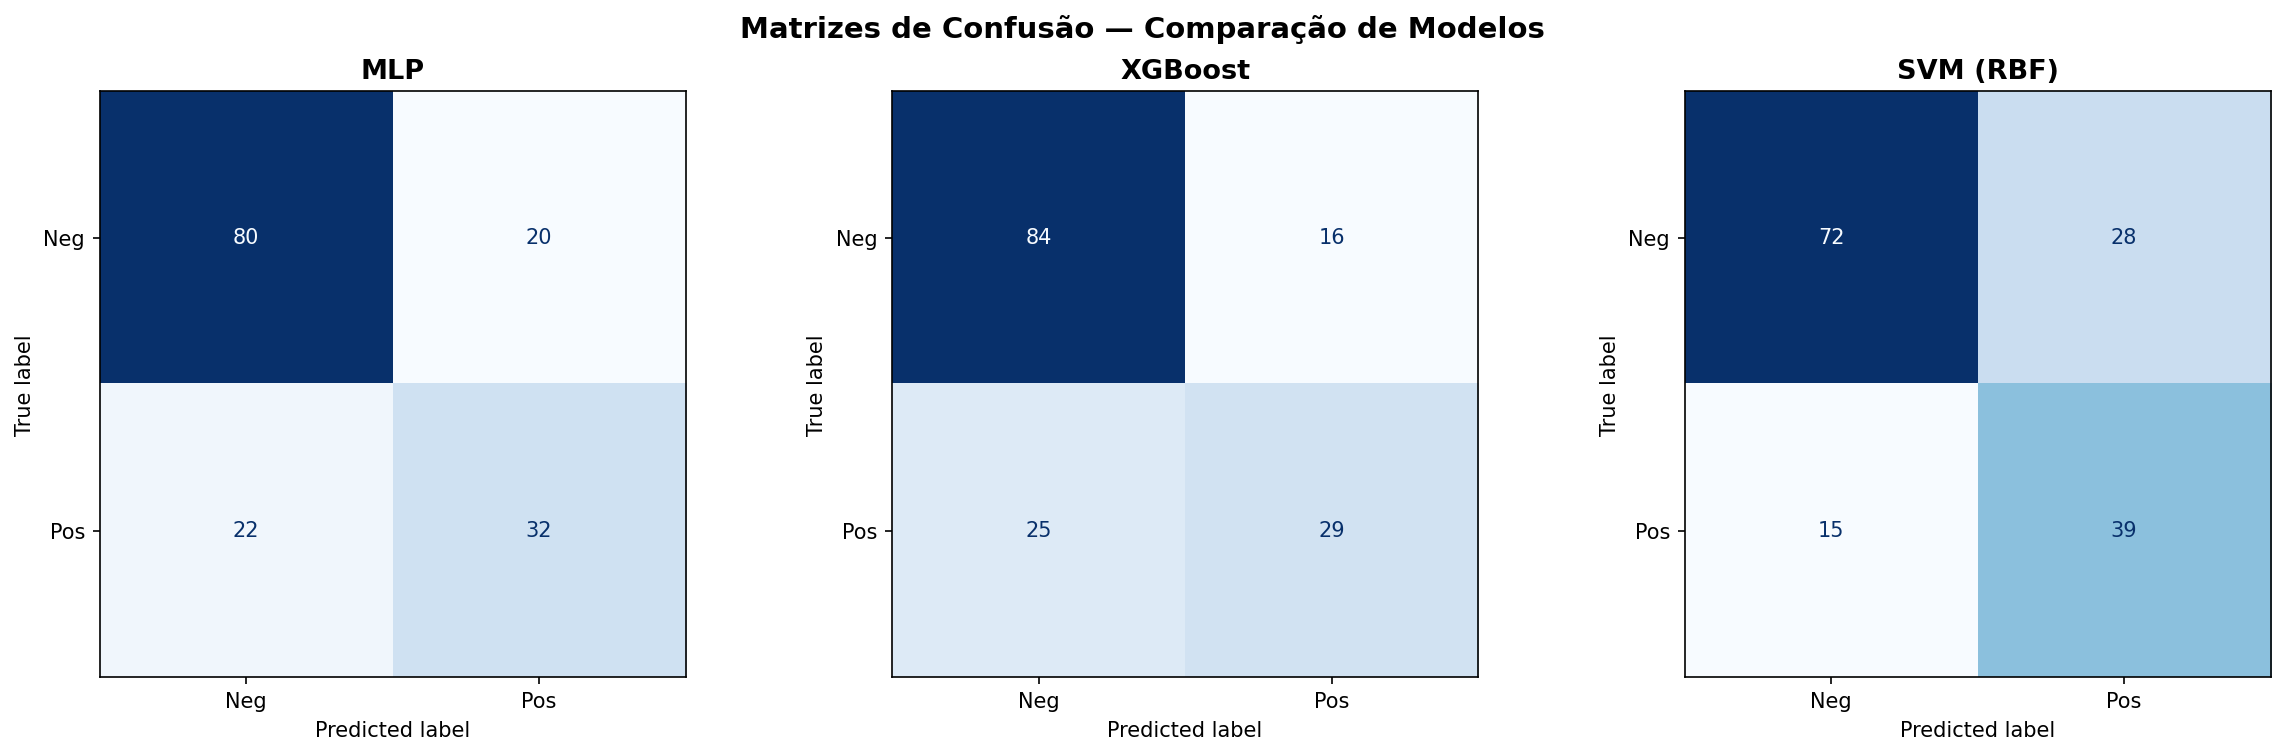
\includegraphics[width=\textwidth]{../output/16_matrizes_confusao.png}
\caption{Matrizes de confusão comparativas: MLP, XGBoost e SVM.}
\end{figure}

\subsubsection{Curvas ROC}

A Figura 17 sobrepõe as curvas ROC dos três modelos. A área sob a curva (AUC) indica a capacidade de discriminação de cada modelo, com valores mais próximos de 1,0 representando melhor desempenho.

\begin{figure}[ht]
\centering
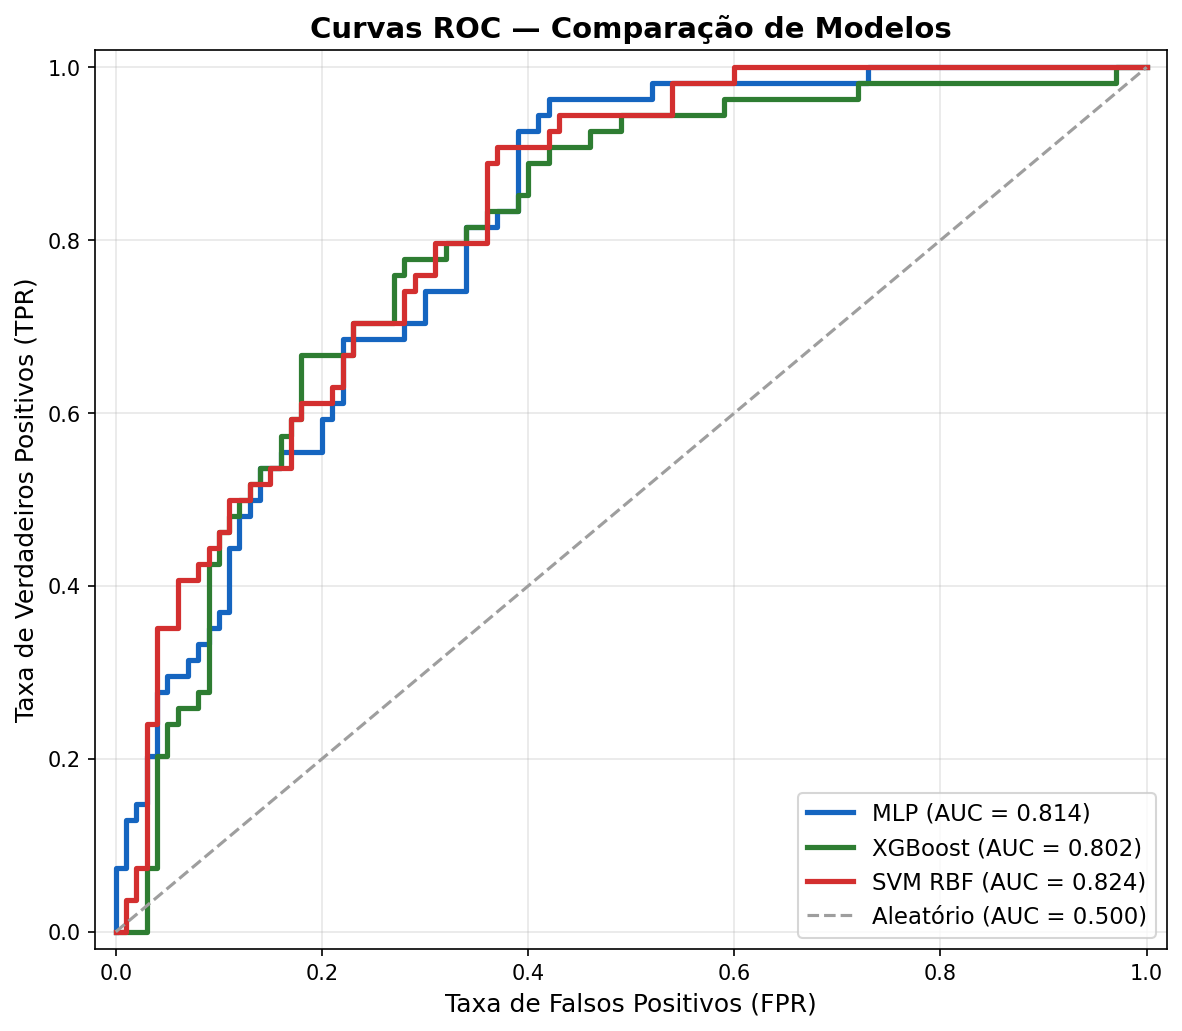
\includegraphics[width=\textwidth]{../output/17_curvas_roc.png}
\caption{Curvas ROC comparativas: MLP, XGBoost e SVM.}
\end{figure}

\subsubsection{Comparação de Métricas}

A Figura 18 sintetiza a comparação de métricas (Accuracy, Precision, Recall, F1-Score e ROC-AUC) entre os três modelos.

\begin{figure}[ht]
\centering
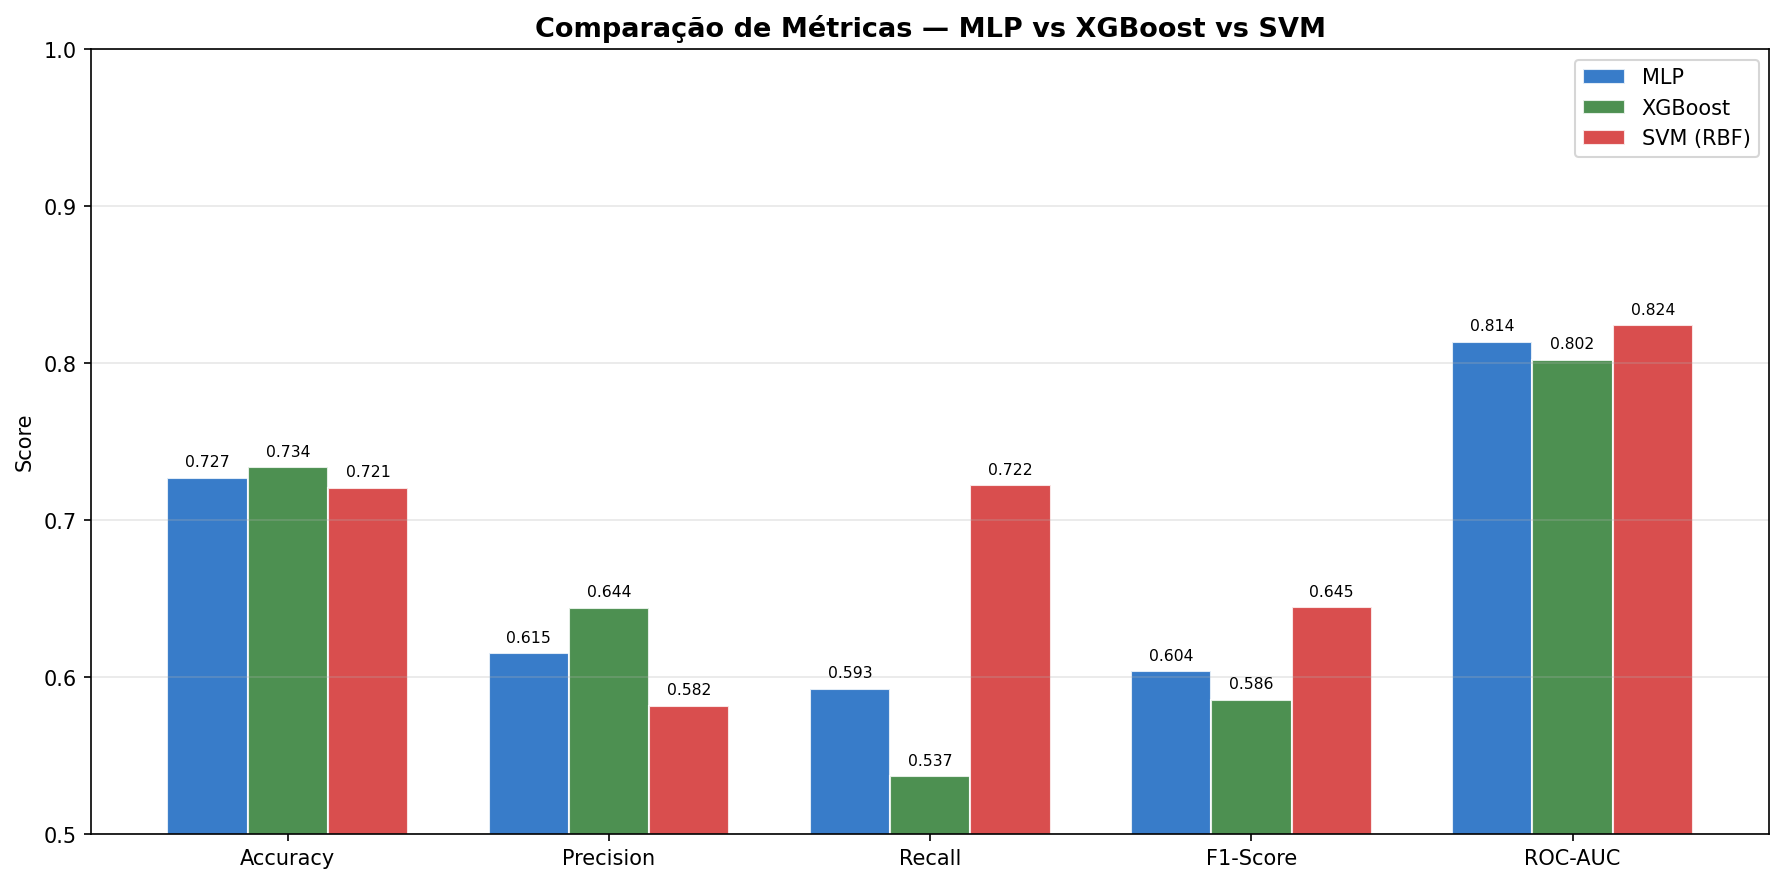
\includegraphics[width=\textwidth]{../output/18_comparacao_metricas_modelos.png}
\caption{Comparação de métricas de classificação: MLP vs. XGBoost vs. SVM.}
\end{figure}

Os três modelos apresentaram desempenho competitivo entre si, com valores de ROC-AUC acima de 0,80 no conjunto de teste. Esse resultado indica que a MLP, apesar de não superar consistentemente os modelos clássicos neste cenário de dados limitados (768 amostras), alcançou desempenho equivalente, validando sua adequação para o problema.

\subsection{Classificação Multiclasse com MLP}

A classificação multiclasse foi realizada com base nos limiares clínicos da ADA para glicose plasmática. A distribuição das classes derivadas é apresentada na Figura 19.

\begin{table}[ht]
\centering
\begin{tabularx}{\textwidth}{|l|X|}
\hline
Classe & Amostras \\
\hline
Normal (< 100 mg/dL) & 212 \\
\hline
Pré-diabético (100--140 mg/dL) & 364 \\
\hline
Diabético ($\geq$ 140 mg/dL) & 192 \\
\hline
\end{tabularx}
\end{table}


\begin{figure}[ht]
\centering
\includegraphics[width=\textwidth]{../output/23_multiclasse_distribuicao.png}
\caption{Distribuição das classes para classificação multiclasse (limiares ADA).}
\end{figure}

As métricas de avaliação no conjunto de teste são apresentadas na tabela a seguir:

\begin{table}[ht]
\centering
\begin{tabularx}{\textwidth}{|l|X|}
\hline
Métrica & Valor \\
\hline
Accuracy & 0,6364 \\
\hline
Precision Macro & 0,6427 \\
\hline
Recall Macro & 0,6359 \\
\hline
F1 Macro & 0,6373 \\
\hline
\end{tabularx}
\end{table}


A Figura 20 exibe a matriz de confusão $3 \times 3$ do modelo multiclasse. Observa-se que a classe "Pré-diabético" apresenta a maior taxa de confusão, o que é esperado por se tratar de uma classe intermediária cujas fronteiras de decisão são limítrofes com as classes adjacentes.

\begin{figure}[ht]
\centering
\includegraphics[width=\textwidth]{../output/24_multiclasse_confusao.png}
\caption{Matriz de confusão da classificação multiclasse (MLP).}
\end{figure}

A Figura 21 apresenta as curvas de aprendizado da MLP multiclasse, evidenciando convergência estável com o early stopping atuando de forma adequada.

\begin{figure}[ht]
\centering
\includegraphics[width=\textwidth]{../output/25_multiclasse_curvas_aprendizado.png}
\caption{Curvas de aprendizado da MLP multiclasse.}
\end{figure}

A Figura 22 resume as métricas obtidas em formato de gráfico de barras.

\begin{figure}[ht]
\centering
\includegraphics[width=\textwidth]{../output/26_multiclasse_metricas.png}
\caption{Métricas de classificação multiclasse (MLP).}
\end{figure}

A Accuracy de 0,64 e o F1 Macro de 0,64 para um problema com 3 classes clinicamente definidas podem ser considerados resultados satisfatórios, particularmente tendo em vista o volume limitado de amostras e a natureza da fronteira entre as classes intermediárias.

\subsection{Regressão com MLP}

As métricas de desempenho da MLP de regressão no conjunto de teste são:

\begin{table}[ht]
\centering
\begin{tabularx}{\textwidth}{|l|X|}
\hline
Métrica & Valor \\
\hline
MAE & 18,6116 mg/dL \\
\hline
MSE & 603,7746 \\
\hline
RMSE & 24,5718 mg/dL \\
\hline
R$^2$ & 0,4165 \\
\hline
\end{tabularx}
\end{table}


O R$^2$ de 0,42 indica que o modelo explica aproximadamente 42\% da variância da concentração de glicose plasmática. O MAE de 18,61 mg/dL representa um erro médio absoluto na unidade clínica original, o que pode ser contextualizado frente à amplitude do intervalo da variável (\texttt{plas} varia de aproximadamente 44 a 199 mg/dL no dataset imputado).

A Figura 23 apresenta, em três painéis, a avaliação do modelo de regressão: (a) valores reais versus preditos, com a linha ideal de referência; (b) análise de resíduos; e (c) curva de aprendizado (loss e R$^2$ por época).

\begin{figure}[ht]
\centering
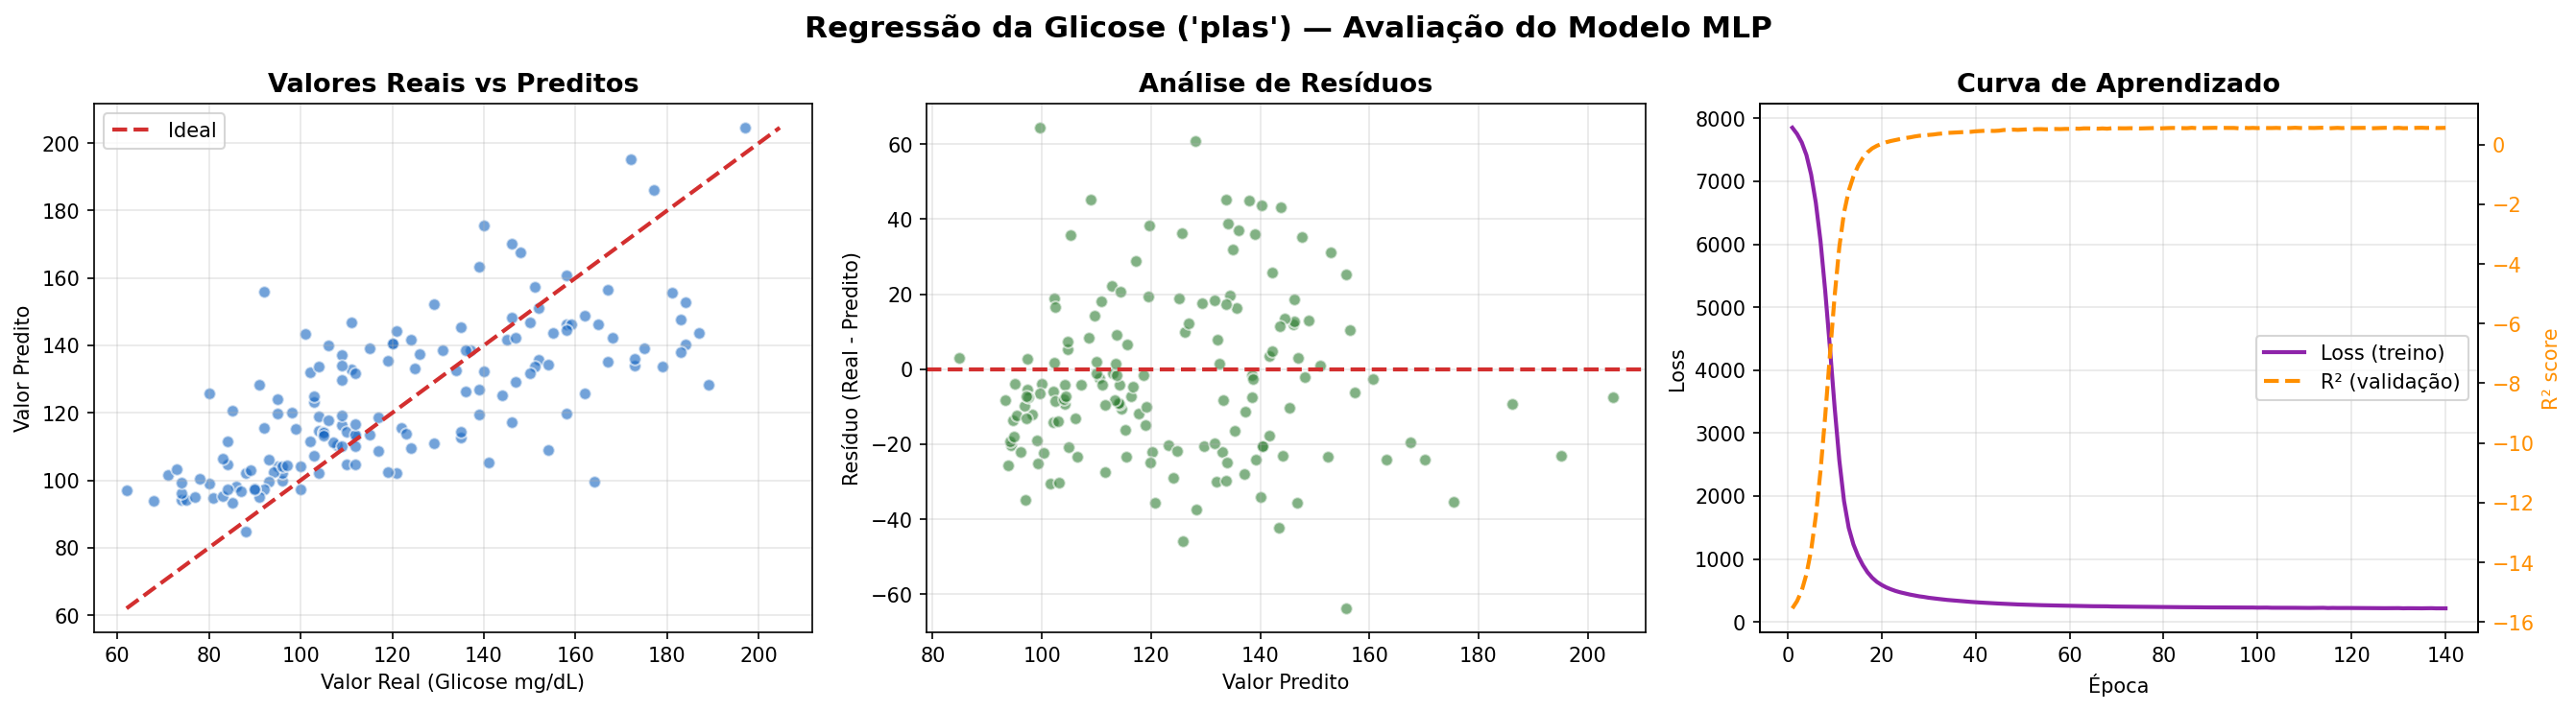
\includegraphics[width=\textwidth]{../output/19_mlp_regressao_avaliacao.png}
\caption{Avaliação da MLP de regressão: valores reais vs. preditos, resíduos e curva de aprendizado.}
\end{figure}

No gráfico de valores reais vs. preditos, observa-se que os pontos se concentram em torno da linha ideal, porém com dispersão considerável nas extremidades (valores de glicose muito baixos ou muito altos), indicando que o modelo tem dificuldade em predizer os casos mais extremos. A análise de resíduos mostra uma distribuição centrada em zero, sem padrões sistemáticos evidentes, o que sugere que o modelo não apresenta viés estrutural significativo. A curva de aprendizado demonstra convergência estável, com o early stopping interrompendo o treinamento no momento adequado.

\subsection{Otimização de Hiperparâmetros com Optuna}

O processo de otimização com Optuna executou 30 trials em aproximadamente 6,9 segundos. Os resultados são sintetizados a seguir:

\textbf{Melhor ROC-AUC obtido via validação cruzada:} 0,8344

\textbf{Melhores hiperparâmetros encontrados:}

\begin{table}[ht]
\centering
\begin{tabularx}{\textwidth}{|l|X|}
\hline
Hiperparâmetro & Valor \\
\hline
Número de camadas & 2 \\
\hline
Neurônios camada 0 & 16 \\
\hline
Neurônios camada 1 & 112 \\
\hline
Taxa de aprendizado & $\approx$ 0,0010 \\
\hline
Função de ativação & relu \\
\hline
Alpha (L2) & $\approx$ 0,0001 \\
\hline
\end{tabularx}
\end{table}


\textbf{Comparação com o modelo original no conjunto de teste:}

\begin{table}[ht]
\centering
\begin{tabularx}{\textwidth}{|l|X|}
\hline
Modelo & ROC-AUC (teste) \\
\hline
MLP Original & 0,7902 \\
\hline
MLP Otimizada & 0,7811 \\
\hline
Delta & $-$0,0091 \\
\hline
\end{tabularx}
\end{table}


A Figura 24 exibe o histórico de otimização do Optuna, mostrando a evolução do valor objetivo (ROC-AUC) ao longo dos 30 trials.

\begin{figure}[ht]
\centering
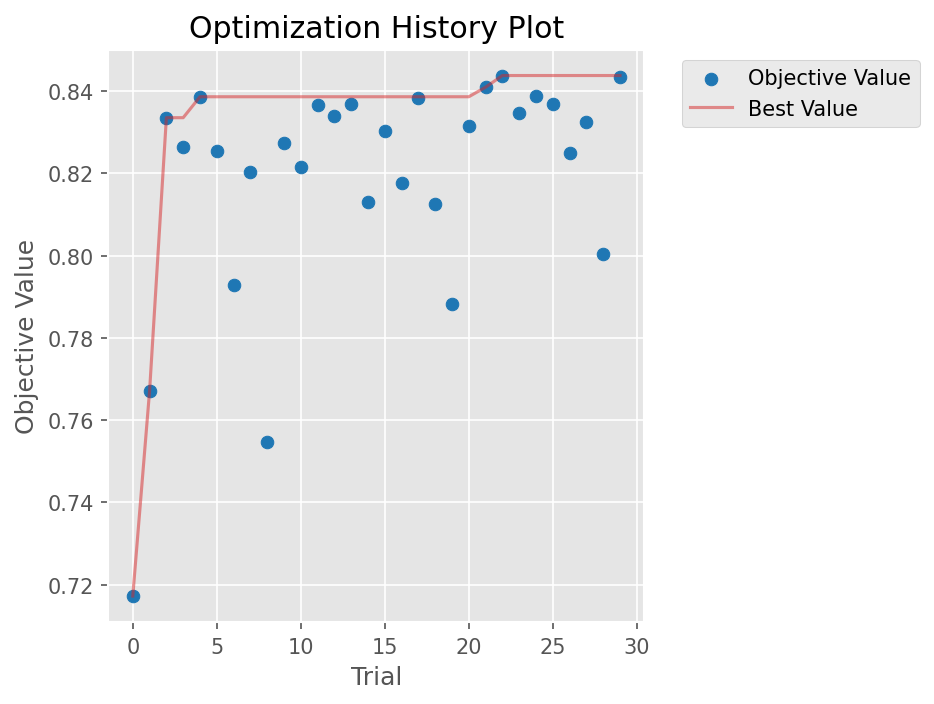
\includegraphics[width=\textwidth]{../output/20_optuna_history.png}
\caption{Histórico de otimização do Optuna.}
\end{figure}

A Figura 25 apresenta a importância dos hiperparâmetros estimada pelo Optuna, indicando quais parâmetros exercem maior influência sobre o desempenho do modelo.

\begin{figure}[ht]
\centering
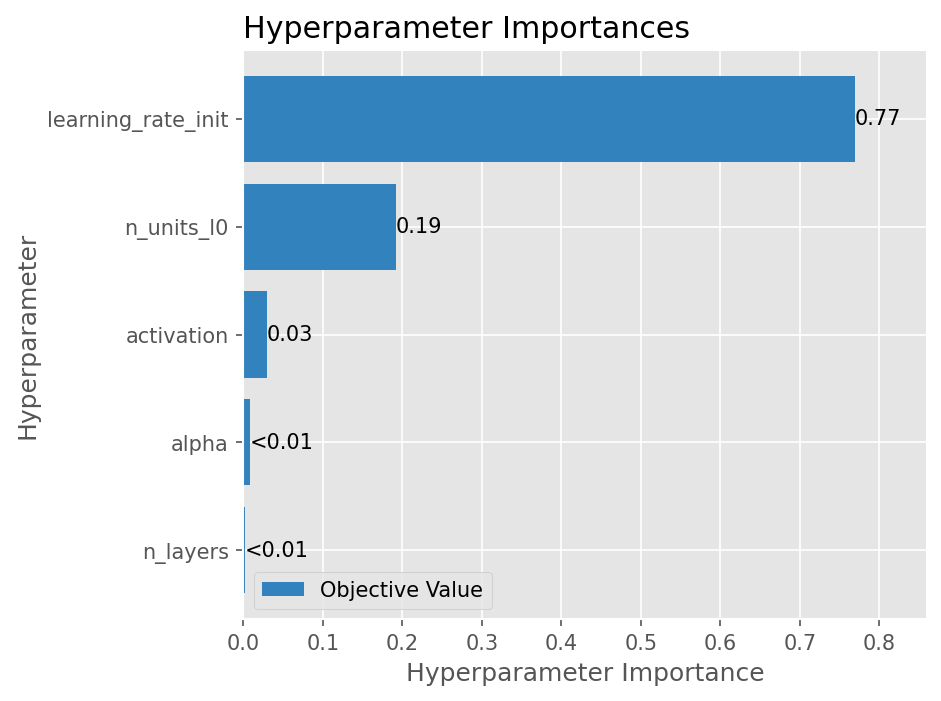
\includegraphics[width=\textwidth]{../output/21_optuna_param_importances.png}
\caption{Importância dos hiperparâmetros estimada pelo Optuna.}
\end{figure}

O delta de $-$0,0091 no ROC-AUC entre o modelo original e o otimizado indica que a configuração inicial da MLP, o que pode indicar variância natural entre os folds de validação e o conjunto de teste final.

\subsection{Regularização e Análise de Overfitting}

A Figura 26 apresenta a comparação das curvas de aprendizado entre o modelo sem regularização (painel esquerdo) e o modelo regularizado (painel direito). No modelo sem regularização, observa-se a métrica de treino (1 $-$ Loss) crescendo de forma contínua enquanto a acurácia de validação estagna, configurando o padrão clássico de overfitting. No modelo regularizado, as curvas de treino e validação permanecem mais próximas, indicando melhor equilíbrio entre ajuste e generalização.

\begin{figure}[ht]
\centering
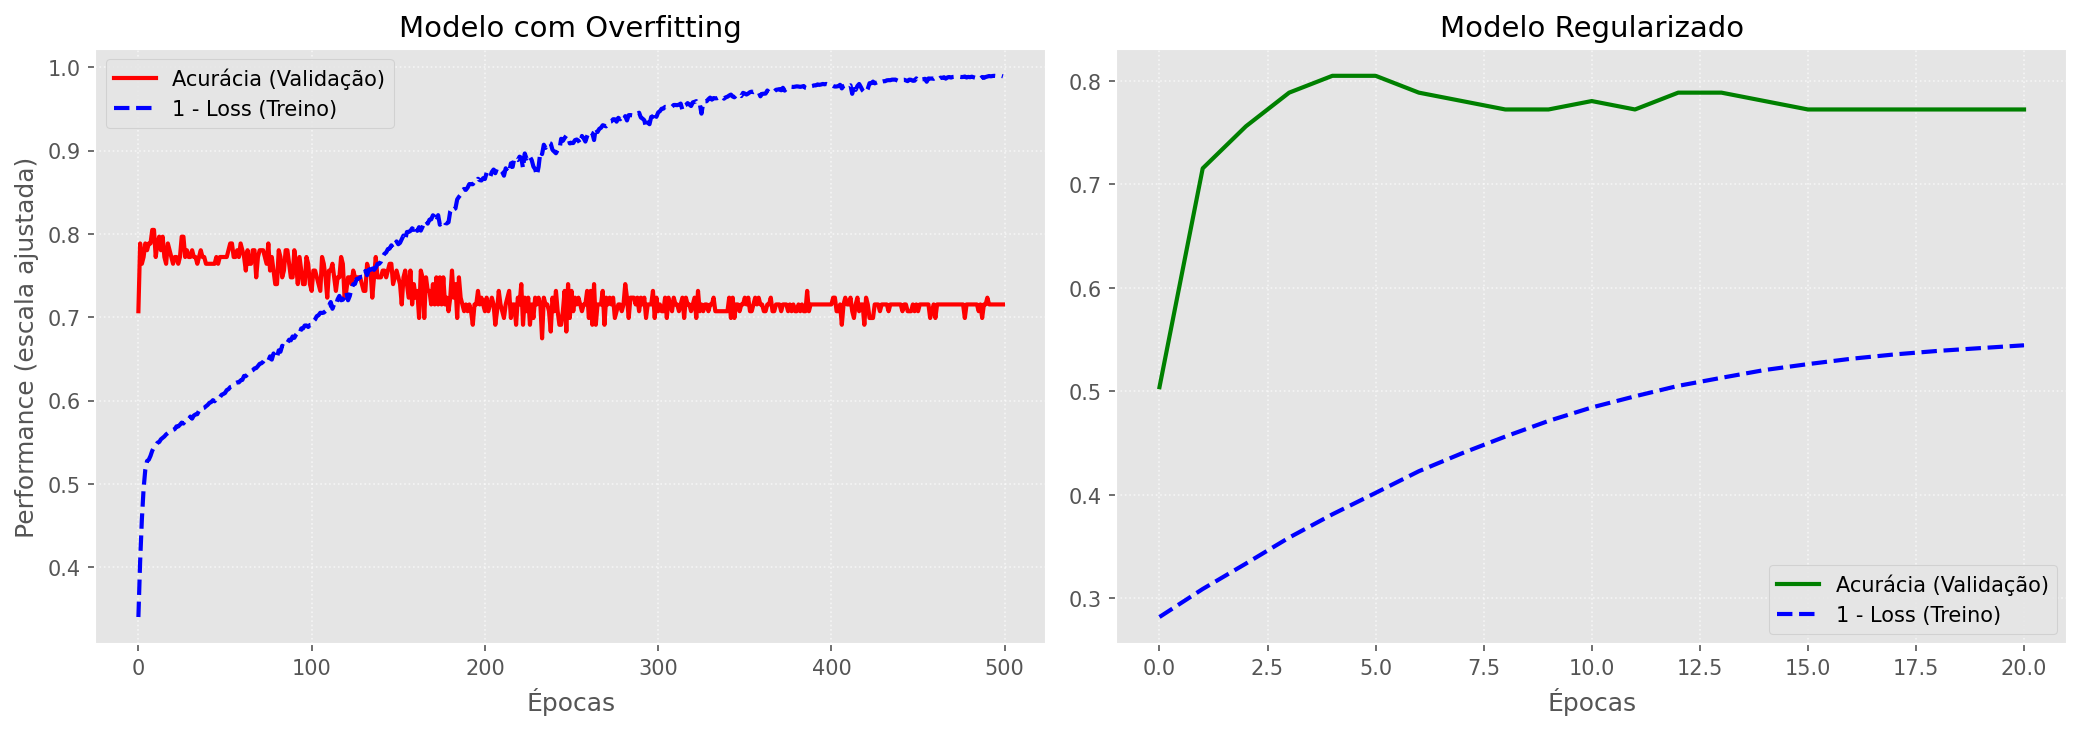
\includegraphics[width=\textwidth]{../output/22_overfitting_comparacao.png}
\caption{Comparação de overfitting: modelo sem regularização vs. modelo regularizado.}
\end{figure}

As métricas comparativas no conjunto de teste são:

\begin{table}[ht]
\centering
\begin{tabularx}{\textwidth}{|l|X|X|X|}
\hline
Métrica & Sem Regularização & Com Regularização & Delta \\
\hline
Accuracy & 0,7078 & 0,7273 & +0,0195 \\
\hline
F1-Score & 0,5361 & 0,5435 & +0,0074 \\
\hline
ROC-AUC & 0,7911 & 0,7896 & $-$0,0015 \\
\hline
\end{tabularx}
\end{table}


\subsubsection{Discussão sobre Overfitting}

\textbf{A rede apresentou sinais de overfitting?}
Sim. O modelo sem regularização (256, 128, 64 neurônios, alpha=0) exibiu o padrão clássico nas curvas de aprendizado: a métrica de treino continuou a subir de forma contínua, enquanto a métrica de validação estagnou e apresentou oscilações, evidenciando o "descolamento" característico entre treino e teste. Esse comportamento confirma que a rede, ao memorizar padrões específicos do conjunto de treino (incluindo ruído e outliers), perdeu capacidade de generalização.

\textbf{Quais técnicas de regularização foram utilizadas?}
Três estratégias foram aplicadas de forma conjunta: (1) simplificação estrutural --- redução das camadas de (256, 128, 64) para (64, 32), diminuindo a capacidade de memorização da rede; (2) regularização L2 com alpha=0,01 --- penalização de pesos elevados, forçando a rede a utilizar pesos menores e mais distribuídos; (3) early stopping com paciência de 15 épocas --- interrupção do treinamento quando a acurácia de validação parou de melhorar.

\textbf{Houve melhoria no desempenho em dados não vistos?}
As métricas no conjunto de teste mostraram melhora no modelo regularizado para Accuracy (+0,0195) e F1-Score (+0,0074), embora tenha havido leve queda no ROC-AUC ($-$0,0015). A análise das curvas de aprendizado mostra que o modelo regularizado apresenta menor gap entre treino e validação, indicando melhor capacidade de generalização e prevenindo quedas abruptas de desempenho em dados inéditos.

\textbf{Qual estratégia apresentou melhor equilíbrio entre desempenho e generalização?}
O modelo regularizado apresentou melhor equilíbrio. Apesar de métricas finais semelhantes, a estabilidade das curvas de treino-validação e a menor tendência a memorização tornam o modelo regularizado preferível em cenários de produção, onde a robustez a dados inéditos é prioritária. A combinação de simplificação estrutural + L2 + early stopping demonstrou eficácia na contenção do overfitting sem degradação significativa do desempenho.

---

\section{Conclusão}

O presente trabalho cumpriu os objetivos propostos ao implementar um pipeline completo de Machine Learning aplicado ao dataset \textit{Pima Indians Diabetes}, abrangendo todas as etapas requisitadas: análise exploratória, pré-processamento, seleção de features, classificação (binária e multiclasse), regressão, otimização de hiperparâmetros e análise de overfitting.

Os principais resultados obtidos podem ser sintetizados da seguinte forma:

\begin{enumerate}
\item \textbf{Pré-processamento:} O KNN Imputer (k=5) e o RobustScaler demonstraram-se adequados para o tratamento do dataset, preservando a estrutura multivariada dos dados e mitigando o impacto de outliers, respectivamente.

\item \textbf{Seleção de features:} A Informação Mútua reduziu o conjunto de 8 para 3 atributos (\texttt{plas}, \texttt{insu}, \texttt{mass}). A seleção foi realizada dentro de cada fold da validação cruzada, eliminando o risco de data leakage. As 3 features foram selecionadas em todos os 10 folds. A análise SHAP corroborou a seleção com concordância muito alta ($\rho$ de Spearman = 0,93, p $<$ 0,001), e o modelo com 3 features manteve desempenho competitivo (ROC-AUC 0,80 vs. 0,83 com todas as features).

\item \textbf{Classificação binária:} A MLP com arquitetura (64, 32, 16) obteve ROC-AUC de 0,7902 no conjunto de teste, desempenho competitivo frente a modelos clássicos e confirmando a capacidade discriminatória com as variáveis selecionadas.

\item \textbf{Classificação multiclasse:} A MLP atingiu Accuracy de 0,6364 e F1 Macro de 0,6373 na categorização de níveis glicêmicos em três classes clínicas (Normal, Pré-diabético e Diabético), resultado considerado satisfatório dado o volume de dados e a natureza limítrofe das fronteiras entre classes.

\item \textbf{Regressão:} O modelo MLP de regressão obteve R$^2$ = 0,42 e MAE = 18,61 mg/dL na predição da glicose plasmática, explicando 42\% da variância da variável alvo. A curva de resíduos não indicou viés sistemático.

\item \textbf{Otimização com Optuna:} A busca por hiperparâmetros (30 trials) resultou em ROC-AUC de validação cruzada de 0,8344, porém sem ganho significativo no conjunto de teste em relação ao modelo original (delta = $-$0,0091). Esse resultado sugere que o desempenho é limitado pelo volume e pela natureza dos dados, e não pela configuração de hiperparâmetros.

\item \textbf{Regularização:} A análise de overfitting confirmou que a rede sem regularização apresentou sinais claros de memorização. A combinação de simplificação estrutural, regularização L2 e early stopping mitigou esse comportamento, melhorando o Accuracy (0,7273 vs 0,7078) e F1-Score no conjunto de teste.

\end{enumerate}
Em suma, o projeto demonstrou que técnicas de aprendizado supervisionado, mesmo em datasets de volume moderado, podem produzir modelos com capacidade discriminativa relevante para o auxílio ao diagnóstico clínico. A integração de métodos de interpretabilidade (SHAP) com a seleção de features (MI) fortaleceu a transparência e a confiabilidade do pipeline, elementos essenciais em aplicações na área de saúde. O resultado global do projeto indica um equilíbrio adequado entre complexidade do modelo, desempenho preditivo e capacidade de generalização.

\end{document}
